%             Exemple d'utilisation de la classe thesul
%             ------------------------------------------
%
%
% (de manière generale, les commandes de thesul sont celles
% qui ne sont pas complètement en minuscules)
%
% Voir la documentation complète pour plus de détails.
%
%
% D. Roegel, 30 mars 2013
%
\documentclass[10pt, oneside]{TUL/thesul}
% \documentclass[12pt]{TUL/thesul}
%----------------------------------------------------------------------
%                     Chargement de quelques packages
%----------------------------------------------------------------------

% Si l'on veut produire une version PDF avec des hyperliens :
% \usepackage[pageanchor=false]{TUL/tulhypref}
\usepackage[hidelinks, pdftex]{TUL/tulhypref}

% Si on veut le style de bibliographie named :
%\usepackage{named}

% Pour les figures :
\usepackage{graphicx}

% Si on veut des mini-tables des matières (utiliser minitoc-hyper 
% en conjonction avec tulhypref) :
\usepackage[french]{minitoc}

\usepackage[backgroundcolor=blue!20!white, linecolor=black]{todonotes}
% \usepackage[disable]{todonotes}
\usepackage{titlesec}
\usepackage{url}
\usepackage{listings}
\usepackage{pstricks}
\usepackage{subfigure}
\usepackage{amsmath}
\usepackage{amsthm}
\usepackage{amssymb}
\usepackage{tabularx}
\usepackage{textcomp}
\usepackage{multirow}

\usepackage[backend=biber, language=french, maxnames=5, citestyle=alphabetic,bibstyle=alphabetic,backref,abbreviate=false,dateabbrev=false,isbn=false,url=false,doi=true]{biblatex}

\addbibresource{these.bib}

% Structure
\newtheorem{pb}{Problème}
\newtheorem{theo}{Théorème}
\newtheorem{defi}{Définition}
\newtheorem{prop}{Proposition}
\newtheorem{pr}{Preuve}
\newtheorem{cor}{Corollaire}
% \theoremstyle{remark}\newtheorem*{preuve}{Preuve}

% % Abbreviations :
\newcommand{\helloworld}{\texttt{Hello World}}
\newcommand{\nasm}{NASM}
\newcommand{\xq}{x86}
\newcommand{\xs}{x86$\_$64}

% Registres
\newcommand{\eax}{\texttt{eax}}
\newcommand{\ebx}{\texttt{ebx}}
\newcommand{\ecx}{\texttt{ecx}}

% Instructions
\newcommand{\mov}{\texttt{mov}}
\newcommand{\cmp}{\texttt{cmp}}
\newcommand{\add}{\texttt{add}}
\newcommand{\jmp}{\texttt{jmp}}
\newcommand{\ret}{\texttt{ret}}
\newcommand{\call}{\texttt{call}}
\newcommand{\push}{\texttt{push}}
\newcommand{\jne}{\texttt{jne}}
\newcommand{\je}{\texttt{je}}

% Sémantique
\newcommand{\BN}{\mathbb N}
\newcommand{\BV}{\mathbb V}
\newcommand{\BX}{\mathbb X}
\newcommand{\BA}{\mathbb A}
\newcommand{\BP}{\mathbb P}
\newcommand{\BT}{\mathbb T}
\newcommand{\BL}{\mathbb L}
\newcommand{\BB}{\mathbb B}
\newcommand{\BNB}{\mathbb N\cup\{\bot\}}
\newcommand{\PN}{\mathcal{P}(\BN)}
\newcommand{\PMN}{\mathcal{P}_M(\BN)}
\newcommand{\Trs}{\mathbb N\cup\{\bot,\top\}}
\newcommand{\TTrs}{\mathcal P(\mathbb V\rightarrow\mathbb N\cup\{\bot,\top\})}
\newcommand{\Tr}{\PN\cup{\top,\bot}}
\newcommand{\TrM}{\PMN\cup\{\top,\bot\}}
\newcommand{\si}{\sigma_{init}}
\newcommand{\specialcell}[2][c]{%
  \begin{tabular}[#1]{@{}l@{}}#2\end{tabular}}

\titleformat{\chapter}[display]
  {\bfseries\huge}
  {\filleft\Large\chaptertitlename~\thechapter}
  {1ex}
  {\titlerule\vspace{1.5ex}\filright}
  [\vspace{1ex}\titlerule]

%-------------------------------------------------------------------
%                             Marges
%-------------------------------------------------------------------

% pour positionner les vraies marges:
%\SetRealMargins{1mm}{1mm}

%-------------------------------------------------------------------
%                             En-têtes
%-------------------------------------------------------------------

% Les en-têtes: quelques exemples
%\UppercaseHeadings 
%\UnderlineHeadings
%\newcommand\bfheadings[1]{{\bf #1}}
%\FormatHeadingsWith{\bfheadings}
%\FormatHeadingsWith{\uppercase}
%\FormatHeadingsWith{\underline}
\newcommand\upun[1]{\uppercase{\underline{\underline{#1}}}}
\FormatHeadingsWith\upun

\newcommand\itheadings[1]{\textit{#1}}
\FormatHeadingsWith{\itheadings}

% pour avoir un trait sous l'en-tete:
\setlength{\HeadRuleWidth}{0.4pt}

%-------------------------------------------------------------------
%                         Les références
%-------------------------------------------------------------------

\NoChapterNumberInRef
\NoChapterPrefix

%-------------------------------------------------------------------
%                           Brouillons
%-------------------------------------------------------------------

% ceci ajoute une marque « brouillon » et la date
%\ThesisDraft

%-------------------------------------------------------------------
%                   Pour collecter un glossaire et un index
%-------------------------------------------------------------------

\makeglossary
\makeindex

\begin{document}





\OddHead={{\leftmark\rightmark}{\hfil\slshape\rightmark}}
\EvenHead={{\leftmark}{{\slshape\leftmark}\hfil}}
\OddFoot={\hfil\thepage}
\EvenFoot={\thepage\hfil}
\pagestyle{ThesisHeadingsII}

%-------------------------------------------------------------------
%                          Encadrements
%-------------------------------------------------------------------

% encadre les chapitres dans la table des matières:
% (ces commandes doivent figurer apres \begin{document}

\FrameChaptersInToc  
%\FramePartsInToc


%-------------------------------------------------------------------
%            Réinitialisation de la numérotation des chapitres
%-------------------------------------------------------------------

% Si la commande suivante est présente,
% elle doit figurer APRÈS \begin{document}
% et avant la première commande \part
% \ResetChaptersAtParts 

%-------------------------------------------------------------------
%               mini-tables des matières par chapitre
%-------------------------------------------------------------------

% préparer les mini-tables des matières par chapitre.
% (commande de minitoc.sty)
\dominitoc

%-------------------------------------------------------------------
%                         Page de titre:
%-------------------------------------------------------------------

\ThesisTitle{Analyse morphologique de logiciels malveillants auto-modifiants}
\ThesisDate{dd/mm/aaaa}
\ThesisAuthor{Aurélien Thierry}

% Type de la these
\ThesisUL

% Jury:

% (ne pas mettre de \\ apres la dernière entree)

% Exemple de création d'une nouvelle catégorie dans le jury:

\NewJuryCategory{family}{\it Membre de la famille :}
                        {\it Membres de la famille :}

\family={Mon frère\\Ma sœur}

\def\blanc{\hspace*{1cm}}

\President    = {Le président}
\Rapporteurs  = {Le rapporteur 1&de Paris\\
                 Le rapporteur 2\\
                 \blanc suite&taratata\\
                 Le rapporteur 3}
\Examinateurs = {L'examinateur 1&d'ici\\
                 L'examinateur 2}
%\Invites=       {}

% Création de la page de titre:
\MakeThesisTitlePage

% on peut en faire plusieurs:
%\MakeThesisTitlePage

%-------------------------------------------------------------------


%-------------------------------------------------------------------
%                          remerciements
%-------------------------------------------------------------------

%\DontFrameThisInToc
\begin{ThesisAcknowledgments}
Merci.
\end{ThesisAcknowledgments}

%-------------------------------------------------------------------
%                            dédicace
%-------------------------------------------------------------------

% \begin{ThesisDedication}
% Ah.
% \end{ThesisDedication}


%-------------------------------------------------------------------
%                  écriture de `Chapitre' et `Partie' 
%                      dans la table des matières
%-------------------------------------------------------------------

\WritePartLabelInToc
\WriteChapterLabelInToc

%-------------------------------------------------------------------
%                        table des matières
%-------------------------------------------------------------------

\tableofcontents

%-------------------------------------------------------------------
%              Exemple d'utilisation de \SpecialSection
%-------------------------------------------------------------------

% \SpecialSection{Introduction générale}


% Pour ne pas avoir le mot « Chapitre » au début de chaque chapitre.
% \NoChapterHead

\DontWriteThisInToc   
\listoffigures


% La commande \mainmatter permet de passer
% à la numérotation arabe (ce que fait \pagenumbering{arabic}) 
% et de faire commencer la nouvelle page 1 sur une page impaire.
% On évitera donc d'utiliser directement \pagenumbering{arabic}.
\mainmatter

\DontFrameThisInToc
\NumberThisInToc
\chapter{Introduction}
Ceci est une introduction.
\todo{Mettre une intro}

% \WriteThisInToc
% \FrameThisInToc
% \NumberThisInToc
\part{Désassemblage et analyse de binaires}

% \NumberThisInToc
\DontFrameThisInToc
\chapter{Assembleur}
% \newcommand{\xqq}{x862}

\todo[inline]{source -> ASM -> binaire // asm -> (désas) -> (décomp)}
Nous nous intéressons en premier lieu aux programmes malveillants fonctionnant sur des ordinateurs personnels.
Les programmes s'exécutant sur ces machines sont compilés afin d'être exécutés nativement dans le langage assembleur spécifique au processeur de la machine.

\section{Compilation et fichiers exécutables}
Un exécutable est en général d'abord écrit dans un langage de haut niveau. Chacun de ses modules est ensuite compilé en un fichier objet (binaire) encodant le langage assembleur spécifique à la machine. La dernière étape est l'édition de liens qui consiste à regrouper tous les fichiers objets en un exécutable unique.

Prenons l'exemple d'un simple \helloworld\ en C (Figure \ref{fig:helloword_c}). Il est uniquement composé d'un appel à la fonction \texttt{printf} permettant l'affichage, à l'exécution, de la chaîne de caractère ``Hello, world.''.
Une implémentation possible en assembleur \nasm\ \xq\ pouvant tourner sous une distribution GNU/Linux est donnée en figure \ref{fig:helloword_asm}. Il est alors composé de deux appels système vers le noyau Linux : une première (sys$\_$write) permettant l'affichage de la chaîne et une seconde (sys$\_$exit) permettant de fermer le processus.
On peut déjà remarquer que le programme est séparé en une section de données (.data) contenant la chaîne de caractère à afficher et une section de code (.text) contenant le code assembleur à exécuter.
\begin{figure}
\begin{lstlisting}[language={C}]
int main(int argc, char* argv[]){
  printf("Hello, world.");
}
\end{lstlisting}
\caption{Code C de \helloworld}
\label{fig:helloword_c}
\end{figure}


\begin{figure}
\begin{lstlisting}[language={[x86masm]Assembler}, escapechar=~]
section .data
msg     db      "Hello, world", 0xa	; ~La chaîne à afficher~
len     equ     $ - msg                 ; ~La taille de la chaîne~

section .text
global _start

_start:
; ~Afficher la chaîne de caractères~
mov     eax, 4      ; ~Numéro d'appel système (sys$\_$write)~
mov     ebx, 1      ; ~Premier argument : le fichier de sortie (ici stdout)~
mov     ecx, msg    ; ~Second argument : un pointeur vers la châine à afficher~
mov	edx, len    ; ~Troisième argument : la taille de la chaîne~
int     0x80        ; ~Appel effectif au noyau~

; ~Fermer proprement le programme~
mov     eax, 1      ; ~Numéro d'appel système (sys$\_$exit)~
mov	ebx, 0	    ; ~Premier argument : le code de retour (0 : normal)~
int     0x80	    ; ~Appel au noyau~
\end{lstlisting}
\caption{Code assembleur \xq\ de \helloworld}
\label{fig:helloword_asm}
\end{figure}

Le fichier binaire exécutable résultant de la compilation est un exécutable binaire pour Linux, sous format ELF.
% Le format ELF est structuré de la manière suivante. 
Comme indiqué sur la figure \ref{fig:structure_elf}, il contient des entêtes dans lesquels sont indiqués des informations générales sur le binaire telle que le point d'entrée du programme, les différentes sections du programme (leur taille, leurs adresses) et les différentes sections : ici une section .data (Figure \ref{fig:data_helloworld}) contient les données du programmes (dont la chaîne de caractères ``Hello World'') et une section .text (Figure \ref{fig:text_helloworld}) contenant le code assembleur à exécuter.
À l'instar de la figure \ref{fig:structure_elf} donnant une structure simplifiée du format ELF pour Linux, la figure \ref{fig:structure_pe} donne un aperçu du format des fichiers exécutables pour un binaire \xq\ sous Windows.

\begin{figure}
\begin{center}
\subfigure[Fichier ELF]{
\begin{tabular}[b]{|c|}
\hline
Entête ELF\\
\hline
Table des entêtes du programme\\
\hline
Section .text\\
\hline
Section .rodata\\
\hline
Section ...\\
\hline
Section .data\\
\hline
Table des sections\\
\hline
\end{tabular}
\label{fig:structure_elf}
}
\subfigure[Fichier PE]{
\begin{tabular}[b]{|c|}
\hline
Entête PE\\
\hline
Table des sections\\
\hline
Sections de code\\
\hline
Sections d'imports\\
\hline
Sections de données\\
\hline
\end{tabular}
\label{fig:structure_pe}
}
\end{center}
\caption{Format des exécutables ELF (Linux) et PE (Windows)}
\label{fig:structure_exe}
\end{figure}

\begin{figure}
\begin{center}
\begin{tabular}{|c|c|l|l|}
\hline
Emplacement dans le fichier & Adresses de chargement & Octets & Caractères ascii\\ 
\hline
94 & 80490a4 & 48 65 6c 6c 6f 2c 20 & H e l l o ,   \\
9b & 80490ab & 77 6f 72 6x 64 & W o r l d \\
a0 & 80490b0 & 0a & Caractère de fin de chaîne       \\
\hline
\end{tabular}
\end{center}
\caption{Section .data de \helloworld}
\label{fig:data_helloworld}
\end{figure}

\begin{figure}
\begin{center}
\begin{tabular}{|c|c|l|l|}
\hline
Emplacement dans le fichier & Adresses de chargement & Octets & Instruction\\ 
\hline
80 & 8048080 & b8 04 00 00 00 & mov    eax,0x4       \\
85 & 8048085 & bb 01 00 00 00 & mov    ebx,0x1       \\
8a & 804808a & b9 a4 90 04 08 & mov    ecx,0x80490a4 \\
8f & 804808f & ba 11 00 00 00 & mov    edx,0x11      \\
94 & 8048094 & cd 80          & int    0x80          \\
96 & 8048096 & bb 00 00 00 00 & mov    ebx,0x0       \\
9b & 804809b & b8 01 00 00 00 & mov    eax,0x1       \\
a0 & 80480a0 & cd 80          & int    0x80          \\
\hline
\end{tabular}
\end{center}
\caption{Section .text de \helloworld}
\label{fig:text_helloworld}
\end{figure}


% \x64
\paragraph{Analyse de binaires}
La principale difficulté lors de l'analyse d'un programme malveillant est que le code source n'est pas disponible à l'analyste qui doit se contenter du fichier binaire compilé.
Un programme compilé se présente donc sous la forme d'un fichier binaire contenant le code machine devant être lancé à l'exécution du programme ainsi que des informations de chargement du binaire : la distinctions de différentes sections (sections de code et sections de données), les adresses mémoires auxquelles le système devra les charger en mémoire ainsi que les librairies du système dont il a besoin et qui devront être chargées.

La principale tâche de l'analyste est alors d'extraire du fichier binaires les quelques informations utiles et surtout d'analyser les parties de code assembleur de l'exécutable.

\section{Assembleur \xq\ et \xs}
L'architecture la plus fréquente sur ces ordinateurs personnels est celle des processeurs Intel CISC avec le jeu d'instructions \xq\ pour les machines adressant la mémoire sur 32 bits, et le jeu d'instructions \xs\ pour celles adressant la mémoire sur 64 bits.
\todo[inline]{
Différence 32 / 64 bits ?
}

\paragraph{Architecture de Harvard modifiée.}
Les ordinateurs actuels fonctionnent selon une version modifiée de l'architecture de Harvard.
La première implémentation de l'architecture de Harvard était L’ASCC (Automatic Sequence Controlled Calculator) d'IBM, également appelé le Mark I et considéré comme le premier calculateur universel, en 1944 \todo{cite autre que wikipedia}. 
Il lisait les instructions sur des cartes perforées et les données étaient entrées manuellement à l'aide d'interrupteurs. 
Ainsi le code exécutable était physiquement non modifiable et séparé des données. 


L'architecture de Von Neumann, qui acceptait la modification de la logique des programmes, était limitée à l'utilisation d'un seul bus de données entre le processeur et la mémoire.
Cette restriction limite grandement les capacités de lecture et écriture mémoire d'une machine utilisant le modèle de Von Neumann. On appelle alors architecture de Harvard modifiée l'architecture de Harvard à plusieurs bus mémoire dans laquelle les instructions et les données sont stockées dans la même mémoire et donc accessibles autant en lecture qu'en écriture.

Dans ce modèle la machine est articulée autour du processeur et de son unité de contrôle chargée de synchroniser les autres composants, d'exécuter les instructions du binaire chargé en mémoire, de gérer les entrées et les sorties, de lire et d'écrire dans la mémoire et les registres. L'unité arithmétique et logique opère toute l'arithmétique du processeur et modifie les registres en conséquence selon les résultats des opérations effectuées. Par exemple si une addition provoque un débordement d'entier, c'est à dire que le résultat de l'addition ne peut être stocké dans un seul registre, alors le registre OF (overflow) est passé à 1.
Une organisation simplifiée d'une machine utilisant le modèle de Harvard modifié est donnée Figure \ref{fig:arch_harvard_mod}.

\paragraph{Structure de la mémoire.}~\\
\todo[inline]{segmentation, pagination? mémoire d'un processus VS mémoire globale?}
En pratique, lors de l'exécution d'un programme, des informations peuvent être stockées en plusieurs lieux. 
Premièrement les registres du processeur permettent un accès rapide à quelques variables.
Certains registres sont réservés, souvent par convention. Par exemple, lors d'un appel de fonction, la convention par défaut en C \todo{cite CDELCL} stipule que la valeur de retour est passé dans le registre \texttt{eax}.
La seconde structure de mémoire est la pile. 
Il s'agit d'une structure de type LIFO (\emph{Last In First Out}) dans laquelle les mots (de 32 bits en \xq, 64 en \xs) sont empilés à l'aide de l'instruction \texttt{push} et dépilés avec l'instruction \texttt{pull} de sorte que le mot dépilé est celui qui a été empilé en dernier.
Les variables locales sont en général enregistrées sur la pile et, lors d'un appel de fonction, les arguments sont passés sur la pile.
La dernière structure est le tas qui est géré par l'appel de fonctions d'allocations dynamiques (telles \texttt{malloc} en C) et est généralement utilisé pour entreposer les structures mémoire plus encombrantes telles que des tableaux ou des structures complexes.
En pratique la mémoire d'un processus contient d'abord les sections de code, puis les sections de données, puis le tas qui est susceptible de s'étendre ainsi que la pile qui peut également s'étendre dans le sens inverse (Figure \ref{fig:mem_process}).
\todo[inline]{Sous windows, sous linux ?}

\begin{figure}
\begin{center}
% 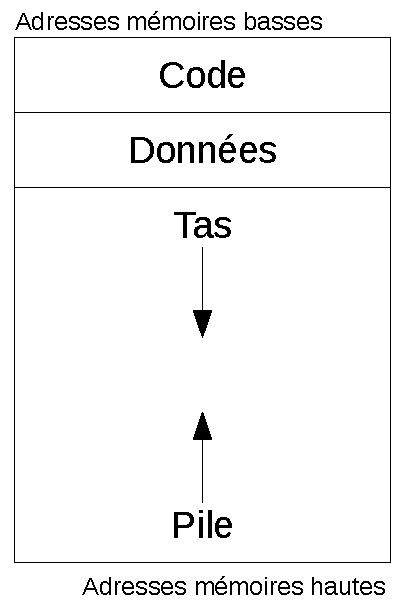
\includegraphics{supports/architecture/pile.pdf}
% % PSTricks TeX macro
% Title: /home/aurelien/RapportsLatex/these/supports/architecture/pile2.dia
% Creator: Dia v0.97.2
% CreationDate: Mon Jun 30 11:09:51 2014
% For: aurelien
% \usepackage{pstricks}
% The following commands are not supported in PSTricks at present
% We define them conditionally, so when they are implemented,
% this pstricks file will use them.
\ifx\setlinejoinmode\undefined
  \newcommand{\setlinejoinmode}[1]{}
\fi
\ifx\setlinecaps\undefined
  \newcommand{\setlinecaps}[1]{}
\fi
% This way define your own fonts mapping (for example with ifthen)
\ifx\setfont\undefined
  \newcommand{\setfont}[2]{}
\fi
\pspicture(-360.050000,-21.152500)(-349.950000,-3.386313)
\psscalebox{1.000000 -1.000000}{
\newrgbcolor{dialinecolor}{0.000000 0.000000 0.000000}%
\psset{linecolor=dialinecolor}
\newrgbcolor{diafillcolor}{1.000000 1.000000 1.000000}%
\psset{fillcolor=diafillcolor}
\psset{linewidth=0.100000cm}
\psset{linestyle=solid}
\psset{linestyle=solid}
\setlinejoinmode{0}
\newrgbcolor{dialinecolor}{1.000000 1.000000 1.000000}%
\psset{linecolor=dialinecolor}
\pspolygon*(-360.000000,5.000000)(-360.000000,20.000000)(-350.000000,20.000000)(-350.000000,5.000000)
\newrgbcolor{dialinecolor}{0.000000 0.000000 0.000000}%
\psset{linecolor=dialinecolor}
\pspolygon(-360.000000,5.000000)(-360.000000,20.000000)(-350.000000,20.000000)(-350.000000,5.000000)
\setfont{Helvetica}{0.800000}
\newrgbcolor{dialinecolor}{0.000000 0.000000 0.000000}%
\psset{linecolor=dialinecolor}
\rput[l](-360.000000,4.000000){\psscalebox{1 -1}{addresses mémoire basses}}
\setfont{Helvetica}{0.800000}
\newrgbcolor{dialinecolor}{0.000000 0.000000 0.000000}%
\psset{linecolor=dialinecolor}
\rput[l](-359.000000,21.000000){\psscalebox{1 -1}{addresses mémoire hautes}}
\psset{linewidth=0.100000cm}
\psset{linestyle=solid}
\psset{linestyle=solid}
\setlinejoinmode{0}
\newrgbcolor{dialinecolor}{1.000000 1.000000 1.000000}%
\psset{linecolor=dialinecolor}
\pspolygon*(-360.000000,5.000000)(-360.000000,7.000000)(-350.000000,7.000000)(-350.000000,5.000000)
\newrgbcolor{dialinecolor}{0.000000 0.000000 0.000000}%
\psset{linecolor=dialinecolor}
\pspolygon(-360.000000,5.000000)(-360.000000,7.000000)(-350.000000,7.000000)(-350.000000,5.000000)
\setfont{Helvetica}{0.800000}
\newrgbcolor{dialinecolor}{0.000000 0.000000 0.000000}%
\psset{linecolor=dialinecolor}
\rput[l](-357.000000,6.000000){\psscalebox{1 -1}{}}
\setfont{Helvetica}{0.800000}
\newrgbcolor{dialinecolor}{0.000000 0.000000 0.000000}%
\psset{linecolor=dialinecolor}
\rput(-355.000000,6.000000){\psscalebox{1 -1}{Code}}
\psset{linewidth=0.100000cm}
\psset{linestyle=solid}
\psset{linestyle=solid}
\setlinejoinmode{0}
\newrgbcolor{dialinecolor}{1.000000 1.000000 1.000000}%
\psset{linecolor=dialinecolor}
\pspolygon*(-360.000000,7.000000)(-360.000000,9.000000)(-350.000000,9.000000)(-350.000000,7.000000)
\newrgbcolor{dialinecolor}{0.000000 0.000000 0.000000}%
\psset{linecolor=dialinecolor}
\pspolygon(-360.000000,7.000000)(-360.000000,9.000000)(-350.000000,9.000000)(-350.000000,7.000000)
\setfont{Helvetica}{0.800000}
\newrgbcolor{dialinecolor}{0.000000 0.000000 0.000000}%
\psset{linecolor=dialinecolor}
\rput[l](-357.000000,8.000000){\psscalebox{1 -1}{}}
\setfont{Helvetica}{0.800000}
\newrgbcolor{dialinecolor}{0.000000 0.000000 0.000000}%
\psset{linecolor=dialinecolor}
\rput(-355.000000,8.000000){\psscalebox{1 -1}{Données}}
\setfont{Helvetica}{0.800000}
\newrgbcolor{dialinecolor}{0.000000 0.000000 0.000000}%
\psset{linecolor=dialinecolor}
\rput(-355.000000,19.221250){\psscalebox{1 -1}{Pile}}
\newrgbcolor{dialinecolor}{1.000000 1.000000 1.000000}%
\psset{linecolor=dialinecolor}
\pspolygon*(-355.505000,9.405000)(-355.505000,10.152500)(-354.495000,10.152500)(-354.495000,9.405000)
\setfont{Helvetica}{0.800000}
\newrgbcolor{dialinecolor}{0.000000 0.000000 0.000000}%
\psset{linecolor=dialinecolor}
\rput(-355.000000,10.000000){\psscalebox{1 -1}{Tas}}
\psset{linewidth=0.100000cm}
\psset{linestyle=dotted,dotsep=0.200000}
\psset{linestyle=dotted,dotsep=0.200000}
\setlinecaps{0}
\newrgbcolor{dialinecolor}{0.000000 0.000000 0.000000}%
\psset{linecolor=dialinecolor}
\psline(-355.000000,11.000000)(-355.000000,12.513197)
\psset{linestyle=solid}
\setlinejoinmode{0}
\setlinecaps{0}
\newrgbcolor{dialinecolor}{0.000000 0.000000 0.000000}%
\psset{linecolor=dialinecolor}
\pspolygon*(-355.000000,12.888197)(-355.250000,12.388197)(-355.000000,12.513197)(-354.750000,12.388197)
\newrgbcolor{dialinecolor}{0.000000 0.000000 0.000000}%
\psset{linecolor=dialinecolor}
\pspolygon(-355.000000,12.888197)(-355.250000,12.388197)(-355.000000,12.513197)(-354.750000,12.388197)
\psset{linewidth=0.100000cm}
\psset{linestyle=dotted,dotsep=0.200000}
\psset{linestyle=dotted,dotsep=0.200000}
\setlinecaps{0}
\newrgbcolor{dialinecolor}{0.000000 0.000000 0.000000}%
\psset{linecolor=dialinecolor}
\psline(-355.000000,18.000000)(-355.000000,16.486803)
\psset{linestyle=solid}
\setlinejoinmode{0}
\setlinecaps{0}
\newrgbcolor{dialinecolor}{0.000000 0.000000 0.000000}%
\psset{linecolor=dialinecolor}
\pspolygon*(-355.000000,16.111803)(-354.750000,16.611803)(-355.000000,16.486803)(-355.250000,16.611803)
\newrgbcolor{dialinecolor}{0.000000 0.000000 0.000000}%
\psset{linecolor=dialinecolor}
\pspolygon(-355.000000,16.111803)(-354.750000,16.611803)(-355.000000,16.486803)(-355.250000,16.611803)
}\endpspicture
\missingfigure{!}
\caption{Organisation de la mémoire d'un processus}
\label{fig:mem_process}
\end{center}
\end{figure}

\begin{figure}
\begin{center}
% Graphic for TeX using PGF
% Title: /home/aurelien/these/supports/architecture/arch.dia
% Creator: Dia v0.97.2
% CreationDate: Wed Jun 18 11:06:57 2014
% For: aurelien
% \usepackage{tikz}
% The following commands are not supported in PSTricks at present
% We define them conditionally, so when they are implemented,
% this pgf file will use them.
\ifx\du\undefined
  \newlength{\du}
\fi
\setlength{\du}{15\unitlength}
\begin{tikzpicture}
\pgftransformxscale{1.000000}
\pgftransformyscale{-1.000000}
\definecolor{dialinecolor}{rgb}{0.000000, 0.000000, 0.000000}
\pgfsetstrokecolor{dialinecolor}
\definecolor{dialinecolor}{rgb}{1.000000, 1.000000, 1.000000}
\pgfsetfillcolor{dialinecolor}
\definecolor{dialinecolor}{rgb}{1.000000, 1.000000, 1.000000}
\pgfsetfillcolor{dialinecolor}
\fill (16.000000\du,5.800000\du)--(16.000000\du,14.300000\du)--(39.000000\du,14.300000\du)--(39.000000\du,5.800000\du)--cycle;
\pgfsetlinewidth{0.100000\du}
\pgfsetdash{}{0pt}
\pgfsetdash{}{0pt}
\pgfsetmiterjoin
\definecolor{dialinecolor}{rgb}{0.000000, 0.000000, 0.000000}
\pgfsetstrokecolor{dialinecolor}
\draw (16.000000\du,5.800000\du)--(16.000000\du,14.300000\du)--(39.000000\du,14.300000\du)--(39.000000\du,5.800000\du)--cycle;
% setfont left to latex
\definecolor{dialinecolor}{rgb}{0.000000, 0.000000, 0.000000}
\pgfsetstrokecolor{dialinecolor}
\node[anchor=west] at (16.450000\du,10.245000\du){};
% setfont left to latex
\definecolor{dialinecolor}{rgb}{0.000000, 0.000000, 0.000000}
\pgfsetstrokecolor{dialinecolor}
\node[anchor=west] at (22.000000\du,7.000000\du){Processeur};
\definecolor{dialinecolor}{rgb}{1.000000, 1.000000, 1.000000}
\pgfsetfillcolor{dialinecolor}
\fill (17.000000\du,8.000000\du)--(17.000000\du,10.000000\du)--(25.000000\du,10.000000\du)--(25.000000\du,8.000000\du)--cycle;
\pgfsetlinewidth{0.100000\du}
\pgfsetdash{}{0pt}
\pgfsetdash{}{0pt}
\pgfsetmiterjoin
\definecolor{dialinecolor}{rgb}{0.000000, 0.000000, 0.000000}
\pgfsetstrokecolor{dialinecolor}
\draw (17.000000\du,8.000000\du)--(17.000000\du,10.000000\du)--(25.000000\du,10.000000\du)--(25.000000\du,8.000000\du)--cycle;
% setfont left to latex
\definecolor{dialinecolor}{rgb}{0.000000, 0.000000, 0.000000}
\pgfsetstrokecolor{dialinecolor}
\node at (21.000000\du,9.206667\du){Unité de contrôle};
\definecolor{dialinecolor}{rgb}{1.000000, 1.000000, 1.000000}
\pgfsetfillcolor{dialinecolor}
\fill (27.000000\du,11.000000\du)--(27.000000\du,13.000000\du)--(38.102500\du,13.000000\du)--(38.102500\du,11.000000\du)--cycle;
\pgfsetlinewidth{0.100000\du}
\pgfsetdash{}{0pt}
\pgfsetdash{}{0pt}
\pgfsetmiterjoin
\definecolor{dialinecolor}{rgb}{0.000000, 0.000000, 0.000000}
\pgfsetstrokecolor{dialinecolor}
\draw (27.000000\du,11.000000\du)--(27.000000\du,13.000000\du)--(38.102500\du,13.000000\du)--(38.102500\du,11.000000\du)--cycle;
% setfont left to latex
\definecolor{dialinecolor}{rgb}{0.000000, 0.000000, 0.000000}
\pgfsetstrokecolor{dialinecolor}
\node at (32.551250\du,12.206667\du){Unité arithmétique et logique};
\definecolor{dialinecolor}{rgb}{1.000000, 1.000000, 1.000000}
\pgfsetfillcolor{dialinecolor}
\fill (28.000000\du,8.000000\du)--(28.000000\du,10.000000\du)--(32.225000\du,10.000000\du)--(32.225000\du,8.000000\du)--cycle;
\pgfsetlinewidth{0.100000\du}
\pgfsetdash{}{0pt}
\pgfsetdash{}{0pt}
\pgfsetmiterjoin
\definecolor{dialinecolor}{rgb}{0.000000, 0.000000, 0.000000}
\pgfsetstrokecolor{dialinecolor}
\draw (28.000000\du,8.000000\du)--(28.000000\du,10.000000\du)--(32.225000\du,10.000000\du)--(32.225000\du,8.000000\du)--cycle;
% setfont left to latex
\definecolor{dialinecolor}{rgb}{0.000000, 0.000000, 0.000000}
\pgfsetstrokecolor{dialinecolor}
\node at (30.112500\du,9.206667\du){Registres};
\pgfsetlinewidth{0.100000\du}
\pgfsetdash{}{0pt}
\pgfsetdash{}{0pt}
\pgfsetbuttcap
{
\definecolor{dialinecolor}{rgb}{0.000000, 0.000000, 0.000000}
\pgfsetfillcolor{dialinecolor}
% was here!!!
\pgfsetarrowsend{stealth}
\definecolor{dialinecolor}{rgb}{0.000000, 0.000000, 0.000000}
\pgfsetstrokecolor{dialinecolor}
\pgfpathmoveto{\pgfpoint{28.000033\du}{8.000024\du}}
\pgfpatharc{306}{235}{2.561783\du and 2.561783\du}
\pgfusepath{stroke}
}
\pgfsetlinewidth{0.100000\du}
\pgfsetdash{}{0pt}
\pgfsetdash{}{0pt}
\pgfsetbuttcap
{
\definecolor{dialinecolor}{rgb}{0.000000, 0.000000, 0.000000}
\pgfsetfillcolor{dialinecolor}
% was here!!!
\pgfsetarrowsend{stealth}
\definecolor{dialinecolor}{rgb}{0.000000, 0.000000, 0.000000}
\pgfsetstrokecolor{dialinecolor}
\pgfpathmoveto{\pgfpoint{27.000016\du}{11.000026\du}}
\pgfpatharc{329}{285}{3.342444\du and 3.342444\du}
\pgfusepath{stroke}
}
\pgfsetlinewidth{0.100000\du}
\pgfsetdash{}{0pt}
\pgfsetdash{}{0pt}
\pgfsetbuttcap
{
\definecolor{dialinecolor}{rgb}{0.000000, 0.000000, 0.000000}
\pgfsetfillcolor{dialinecolor}
% was here!!!
\pgfsetarrowsend{stealth}
\definecolor{dialinecolor}{rgb}{0.000000, 0.000000, 0.000000}
\pgfsetstrokecolor{dialinecolor}
\pgfpathmoveto{\pgfpoint{24.999562\du}{9.999435\du}}
\pgfpatharc{143}{128}{11.225061\du and 11.225061\du}
\pgfusepath{stroke}
}
\definecolor{dialinecolor}{rgb}{1.000000, 1.000000, 1.000000}
\pgfsetfillcolor{dialinecolor}
\fill (18.000000\du,2.503333\du)--(18.000000\du,4.450000\du)--(22.045000\du,4.450000\du)--(22.045000\du,2.503333\du)--cycle;
\pgfsetlinewidth{0.100000\du}
\pgfsetdash{}{0pt}
\pgfsetdash{}{0pt}
\pgfsetmiterjoin
\definecolor{dialinecolor}{rgb}{0.000000, 0.000000, 0.000000}
\pgfsetstrokecolor{dialinecolor}
\draw (18.000000\du,2.503333\du)--(18.000000\du,4.450000\du)--(22.045000\du,4.450000\du)--(22.045000\du,2.503333\du)--cycle;
% setfont left to latex
\definecolor{dialinecolor}{rgb}{0.000000, 0.000000, 0.000000}
\pgfsetstrokecolor{dialinecolor}
\node at (20.022500\du,3.683333\du){Mémoire};
\definecolor{dialinecolor}{rgb}{1.000000, 1.000000, 1.000000}
\pgfsetfillcolor{dialinecolor}
\fill (18.000000\du,16.000000\du)--(18.000000\du,18.000000\du)--(22.000000\du,18.000000\du)--(22.000000\du,16.000000\du)--cycle;
\pgfsetlinewidth{0.100000\du}
\pgfsetdash{}{0pt}
\pgfsetdash{}{0pt}
\pgfsetmiterjoin
\definecolor{dialinecolor}{rgb}{0.000000, 0.000000, 0.000000}
\pgfsetstrokecolor{dialinecolor}
\draw (18.000000\du,16.000000\du)--(18.000000\du,18.000000\du)--(22.000000\du,18.000000\du)--(22.000000\du,16.000000\du)--cycle;
% setfont left to latex
\definecolor{dialinecolor}{rgb}{0.000000, 0.000000, 0.000000}
\pgfsetstrokecolor{dialinecolor}
\node at (20.000000\du,17.206667\du){Entrées};
\definecolor{dialinecolor}{rgb}{1.000000, 1.000000, 1.000000}
\pgfsetfillcolor{dialinecolor}
\fill (24.000000\du,16.000000\du)--(24.000000\du,18.000000\du)--(28.000000\du,18.000000\du)--(28.000000\du,16.000000\du)--cycle;
\pgfsetlinewidth{0.100000\du}
\pgfsetdash{}{0pt}
\pgfsetdash{}{0pt}
\pgfsetmiterjoin
\definecolor{dialinecolor}{rgb}{0.000000, 0.000000, 0.000000}
\pgfsetstrokecolor{dialinecolor}
\draw (24.000000\du,16.000000\du)--(24.000000\du,18.000000\du)--(28.000000\du,18.000000\du)--(28.000000\du,16.000000\du)--cycle;
% setfont left to latex
\definecolor{dialinecolor}{rgb}{0.000000, 0.000000, 0.000000}
\pgfsetstrokecolor{dialinecolor}
\node at (26.000000\du,17.206667\du){Sorties};
\pgfsetlinewidth{0.100000\du}
\pgfsetdash{}{0pt}
\pgfsetdash{}{0pt}
\pgfsetbuttcap
{
\definecolor{dialinecolor}{rgb}{0.000000, 0.000000, 0.000000}
\pgfsetfillcolor{dialinecolor}
% was here!!!
\pgfsetarrowsend{stealth}
\definecolor{dialinecolor}{rgb}{0.000000, 0.000000, 0.000000}
\pgfsetstrokecolor{dialinecolor}
\pgfpathmoveto{\pgfpoint{19.011333\du}{4.449795\du}}
\pgfpatharc{202}{159}{4.783839\du and 4.783839\du}
\pgfusepath{stroke}
}
\pgfsetlinewidth{0.100000\du}
\pgfsetdash{}{0pt}
\pgfsetdash{}{0pt}
\pgfsetbuttcap
{
\definecolor{dialinecolor}{rgb}{0.000000, 0.000000, 0.000000}
\pgfsetfillcolor{dialinecolor}
% was here!!!
\pgfsetarrowsend{stealth}
\definecolor{dialinecolor}{rgb}{0.000000, 0.000000, 0.000000}
\pgfsetstrokecolor{dialinecolor}
\pgfpathmoveto{\pgfpoint{20.999967\du}{8.000604\du}}
\pgfpatharc{4}{-33}{5.798338\du and 5.798338\du}
\pgfusepath{stroke}
}
\pgfsetlinewidth{0.100000\du}
\pgfsetdash{}{0pt}
\pgfsetdash{}{0pt}
\pgfsetbuttcap
{
\definecolor{dialinecolor}{rgb}{0.000000, 0.000000, 0.000000}
\pgfsetfillcolor{dialinecolor}
% was here!!!
\pgfsetarrowsend{stealth}
\definecolor{dialinecolor}{rgb}{0.000000, 0.000000, 0.000000}
\pgfsetstrokecolor{dialinecolor}
\pgfpathmoveto{\pgfpoint{19.000096\du}{9.999695\du}}
\pgfpatharc{198}{144}{6.720258\du and 6.720258\du}
\pgfusepath{stroke}
}
\pgfsetlinewidth{0.100000\du}
\pgfsetdash{}{0pt}
\pgfsetdash{}{0pt}
\pgfsetbuttcap
{
\definecolor{dialinecolor}{rgb}{0.000000, 0.000000, 0.000000}
\pgfsetfillcolor{dialinecolor}
% was here!!!
\pgfsetarrowsend{stealth}
\definecolor{dialinecolor}{rgb}{0.000000, 0.000000, 0.000000}
\pgfsetstrokecolor{dialinecolor}
\pgfpathmoveto{\pgfpoint{26.000003\du}{16.000021\du}}
\pgfpatharc{353}{315}{10.161156\du and 10.161156\du}
\pgfusepath{stroke}
}
\pgfsetlinewidth{0.100000\du}
\pgfsetdash{}{0pt}
\pgfsetdash{}{0pt}
\pgfsetbuttcap
{
\definecolor{dialinecolor}{rgb}{0.000000, 0.000000, 0.000000}
\pgfsetfillcolor{dialinecolor}
% was here!!!
\pgfsetarrowsend{stealth}
\definecolor{dialinecolor}{rgb}{0.000000, 0.000000, 0.000000}
\pgfsetstrokecolor{dialinecolor}
\pgfpathmoveto{\pgfpoint{24.999678\du}{8.199859\du}}
\pgfpatharc{114}{78}{4.877392\du and 4.877392\du}
\pgfusepath{stroke}
}
\pgfsetlinewidth{0.100000\du}
\pgfsetdash{}{0pt}
\pgfsetdash{}{0pt}
\pgfsetbuttcap
{
\definecolor{dialinecolor}{rgb}{0.000000, 0.000000, 0.000000}
\pgfsetfillcolor{dialinecolor}
% was here!!!
\pgfsetarrowsend{stealth}
\definecolor{dialinecolor}{rgb}{0.000000, 0.000000, 0.000000}
\pgfsetstrokecolor{dialinecolor}
\pgfpathmoveto{\pgfpoint{33.300602\du}{10.953459\du}}
\pgfpatharc{18}{-64}{2.044555\du and 2.044555\du}
\pgfusepath{stroke}
}
\end{tikzpicture}

\caption{Architecture de Harvard modifiée}
\label{fig:arch_harvard_mod}
\end{center}
\end{figure}

\paragraph{Jeu d'instructions.}
\todo{notation intel?}
Les processeurs Intel \xq\ utilisent un jeu d'instruction complexe (CISC). La représentation d'une instruction en une suite d'octets inclut principalement un type opération (opcode\todo{opcode?}) et ses arguments. Des informations supplémentaire peuvent être codées dans l'instruction, comme des préfixes. Le format des instructions détaillé est donné figure \ref{fig:format_insts_x86}.
L'instruction \texttt{mov ecx, 0x080490a4} de la figure \ref{fig:text_helloworld}, codée sur \texttt{b9 a4 90 04 08} est composée de l'opcode \texttt{b8+r} indiquant une opération de copie d'une valeur immédiate vers un registre. Ici le modificateur r est égal à 1, ce qui indique que le registre concerné est ecx. La valeur à copier vers le registre est 0x080490a4 soient les octets \texttt{a4 90 04 08} codés en petit-boutistes \todo{endianness ??}, c'est à dire que les mots de poids faibles sont écrits en premiers, à l'inverse de l'écriture usuelle.
Il s'agit d'une assignation immédiate et la valeur à copier vers \texttt{ecx} est la valeur immédiate.
Le décalage permet de modifier une instruction d'adressage indirect comme \texttt{mov ecx, [eax]}, écrivant le contenu en mémoire à l'adresse \texttt{eax} dans le registre \texttt{ecx} en \texttt{mov ebx, [eax+d]} où \texttt{d} est le décalage.
Enfin les préfixes permettent par exemple de répéter plusieurs fois l'instruction jusqu'à ce qu'une condition sur un registre soit remplie.

\begin{figure}
\begin{center} 
\begin{tabular}{|c|c|c|c|c|c|}
\hline
% Prefixe & Opcode & Modificateur & SIB & Déplacement d'octet & Adressage\\
% 1 à 4 & 1 à 3 & 0 ou 1 & 0 ou 1 & 0 à 4 & 0 à 4\\
Prefixe & Opcode & Modificateur & Décalage & Valeur immédiate\\
1 à 4 & 1 à 3 & 0 à 2 & 0 à 4 & 0 à 4\\
\hline
\end{tabular}
\end{center} 
\caption{Format d'une instruction \xq}
\label{fig:format_insts_x86}
\end{figure}

\paragraph{Intuition de sémantique.}
% ~\\
% \todo[inline]{assignations (déplacement en mémoire)\\
% opérations arithmétique\\
% controle de flot inconditionnel\\
% conditionnel}
% 
% \todo[inline]{effets de bords\\
% explicites\\
% implicites}

Bien que la documentation exhaustive d'Intel pour les processeurs \xq\ et \xs\ \cite{intel_vol2} détaille plusieurs centaines d'instructions, elles peuvent être regroupées en 3 classes.
Prenons l'instruction \texttt{mov}. Elle sert à copier des informations depuis une zone (mémoire ou registre) vers une autre zone.
Ainsi \texttt{mov eax, [ebx+10]} copie la valeur à l'adresse \texttt{ebx+10} dans le registre \eax. 
Cette instruction est déclinée en plusieurs dizaines de variantes selon la taille et le type des opérandes copiés.

Une seconde catégorie d'instructions permet de gérer les opérations arithmétiques sur les octets en mémoire et dans les registres.
Une instructions comme \texttt{add eax, ebx} ajoute la valeur de \ebx\ à celle de \eax\ et stocke le résultat de l'opération dans \eax.
Ce type d'opération combine en fait une opération arithmétique et une assignation. 
On peut y inclure l'instruction \cmp\ qui compare deux valeurs et met à jour les registres de tests. 
Ces registres indiquent entre autres si le signe du résultat d'une opération ainsi que si elle a provoqué un débordement d'entier (dans le cas où le résultat est trop grand pour être stocké sur un entier).
En fait les instructions arithmétiques comme \add\ provoquent aussi une mise à jour de ces registres : il s'agit d'une assignation implicite.

Les instructions précédemment décrites sont séquentielles et ne modifient pas l'ordre d'exécution d'une instruction. 
Après l'exécution d'une instruction de type \mov\ à l'adresse $a$ codée sur $n$ octets, l'instruction située à l'adresse $a+n$.
Le dernier type d'instruction modifie le flot de contrôle du programme et effectuent des sauts à des adresses spécifiées dans le programme.
Ces sauts peuvent être inconditionnels comme un \texttt{jmp 8048085} qui provoque un saut à l'adresse \texttt{8048085} ou le saut dynamique \texttt{jmp eax} dont l'adresse cible du saut est la valeur de \eax.
Les sauts peuvent aussi être conditionnels : \texttt{je +10}, à l'adresse $a$ et de taille $n$, sera suivie de l'instruction à l'adresse $a+10$ si le registre ZF vaut 1 (en cas d'égalité) et de l'instruction à l'adresse $a+n$ dans le cas contraire.


\section{Désassemblage}
Le désassemblage est l'opération inverse de l'assemblage : il consiste à récupérer le code assembleur source du binaire.
Cette tâche semble particulièrement simple puisque l'assemblage consiste simplement à trouver les octets correspondants à chaque instruction à l'aide de la documentation officielle du processeur puis à mettre en forme le fichier binaire en remplissant correctement ses entêtes et ses sections.
Pourtant on a vu que, dans le modèle d'Harvard modifié, les données et le code peuvent être mêlés. 
En particulier les parties de données (comme la section .data) peuvent être exécutées. 
De même les sections de code peuvent contenir des informations destinées à être simplement lues ou modifiées mais jamais exécutées.
La difficulté du désassemblage consiste donc à séparer les parties potentiellement exécutables des données.

Ainsi un désassemblage à priori cohérent de \helloworld\ consisterait à considérer les deux sections comme contenant du code potentiellement exécutable. Ce désassemblage sera composé de la section .text déjà désassemblé Figure \ref{fig:text_helloworld} et la section .data donnée Figure \ref{fig:data_exec_helloworld}.
Ce désassemblage n'est pas correct et on peut le prédire. 
On connaît le point d'entrée du binaire, qui est l'adresse \texttt{8048080} dans la section .text.
Les instructions exécutées dans la section .text à la suite du point d'entrée sont séquentielles et ne peuvent détourner l'exécution vers la section .data. 
Le code désassemblé dans cette section n'est donc pas atteignable. Dans ce cas on sait alors que la section .data ne contient pas de code et ne doit pas être désassemblée.

\paragraph{Utilisation de sauts dynamiques.}
En pratique un programme est constitué d'un grand nombre d'instructions de saut et notamment de sauts dynamiques de type \texttt{jmp eax}.
Ce type d'instructions posent un souci lors de l'analyse : sans connaître précisément la ou les valeurs potentielles d'\eax, impossible de prédire la cible du saut et donc de savoir le code potentiellement exécuté à la suite de cette instruction.
Dans l'exemple du \helloworld, si une telle instruction est présente dans la section .text, il devient difficile d'exclure l'exécution possible de code dans la section .data.

\paragraph{Difficulté théorique du désassemblage.}
On a vu que le problème du désassemblage tient dans la difficulté de séparer les parties de code potentiel des parties de données.
Plus précisément le but du désassemblage d'un programme P est alors de déterminer l'ensemble des adresses $a$ du programme pour lesquelles il existe une entrée I telle que l'exécution de P(I) atteint $a$.
Nous citons ici un argument tiré de la thèse de Joan Calvet \cite{Calvet2013} montrant le caractère indécidable de ce problème en réduisant le problème de l'arrêt à celui-ci.

Supposons que le problème soit décidable et notons, pour tout programme P, $CODE(P)$ l'ensemble des adresses des instructions de P atteignables lors de l'exécution de P. Pour tout programme P et toute entrée I à P, on peut définir le programme P' suivant qui ne prend pas d'entrée :

\begin{center}
\begin{tabular}{|l|l|}
\hline
Adresse & Commande \\
\hline
0 & call P(I)\\
$\alpha$ & halt \\
\hline
\end{tabular}
\end{center}

Deux cas sont alors possibles.
\begin{itemize}
 \item Soit $\alpha\in\ CODE(P')$ et dans ce cas l'exécution atteint l'adresse $\alpha$ donc le programme P termine sur l'entrée I.
 \item Soit $\alpha\notin\ CODE(P')$ donc le programme P ne termine pas sur l'entrée I.
\end{itemize}
~\\
On en déduit donc que le désassemblage permet de résoudre le problème de l'arrêt qui est pourtant connu pour être indécidable ; c'est absurde.
Ainsi le problème du désassemblage est indécidable.


\begin{figure}
\begin{center}
\begin{tabular}{|c|c|l|l|}
\hline
Emplacement dans le fichier & Adresses de chargement & Octets & Instruction\\ 
\hline
94 & 80490a4 & 48    & dec    eax			\\
95 & 80490a5 & 65    & gs				\\
96 & 80490a6 & 6c    & ins    BYTE PTR es:[edi],dx	\\
97 & 80490a7 & 6c    & ins    BYTE PTR es:[edi],dx	\\
98 & 80490a8 & 6f    & outs   dx,DWORD PTR ds:[esi]	\\
99 & 80490a9 & 2c 20 & sub    al,0x20			\\
9b & 80490ab & 77 6f & ja     0x804911c			\\
9d & 80490ad & 72 6c & jb     0x804911b			\\
9f & 80490af & 64    & fs				\\
a0 & 80490b0 & 0a    & .byte 0xa			\\
\hline
\end{tabular}
\end{center}
\caption{Section .data de \helloworld\ désassemblée comme du code}
\label{fig:data_exec_helloworld}
\end{figure}

\todo[inline]{Analyse statique, analyse dynamique ?\\
linear sweep, recursive traversal, speculative disassembly}

\subsection{Analyse statique}
\paragraph{Linear sweep.}
\paragraph{Recursive disassembly.}

\subsection{Analyse dynamique}

% \paragraph{Décompilation.}

\section{Obfuscations}
\subsection{Auto-modification}
\todo[inline]{
Qu'est-ce ? \\
Autorisé par l'OS (NX ?) \\
Comment ? \\
Exemple
}

\subsection{Obscurcissement statique}
\todo[inline]{
Ajout de junk code \\
Détournement de calls \\
Chevauchements \\
Prédicats opaques\\
}
\todo[inline]{
Réorganisation du code \\
Aplatissement de CFG \\
}

% \section{Difficulté calculatoire de l'analyse de binaire}
% \subsection{Désassemblage}
% \subsection{Décompilation}

\DontFrameThisInToc
\chapter{Analyse dynamique}
\todo[inline]{Problème des entrées, comment gérer SM ?}
L'analyse dynamique consiste à se baser sur une ou des exécutions particulières d'un programme pour inférer des propriétés sur son fonctionnement.
Elle demande donc de se munir d'une langage modélisant le fonctionnement de la machine durant l'exécution du programme, d'une sémantique concrète de l'assembleur utilisé et de lancer l'évaluation sémantique du programme sur une ou plusieurs entrées.
Les entrées d'un programme sont par exemple les paramètres passés lors de l'appel au programme, l'état de la machine lors du démarrage, les données lues depuis la mémoire et les saisies faites par l'utilisateur au clavier ou à la souris lors de l'exécution s'il s'agit d'une application dotée d'une interface graphique.



\section{Sémantique concrète pour un langage assembleur}
% \section{Sémantique}
\paragraph{Représentation de la mémoire et des registres.}
On peut voir la mémoire comme un tableau contenant la pile et le tas, indexés sur les entiers. Les registres sont des variables distinctes de la mémoire et sont en nombre limité. Enfin, pour pouvoir gérer l'adressage indirect : \texttt{[eax]} fait référence à la valeur en mémoire à l'adresse contenue dans \eax, on ajoute les pointeurs vers une variable. Ces éléments sont définis formellement à la définition \ref{def:sem_conc_var}.

\begin{rem}
 Avec cette définition, une valeur en mémoire peut pointer vers un registre. De même un registre peut pointer vers un autre registre.
 Ces deux possibilités ne sont pas réalisables avec l'assembleur \xq\ ou \xs.
\end{rem}


\begin{defi}
On définit les symboles $x\in\BX$ comme constitués de variables $v\in\BV$ et de pointeurs $p\in\BP$ vers des variables. $\BV$ contient un ensemble fini de registres $a\in\BA$ et un tableau de taille finie $\BT=\textlbrackdbl 0,\ T\textrbrackdbl$. Les éléments de $\BP$ sont des pointeurs vers une variable : $\{[v],\ v\in \BV\}$.
Les valeurs possibles pour les variables sont dans $\BN$.
\label{def:sem_conc_var}
\end{defi}

Le langage assembleur est très simple du point de vue de la sémantique. Il peut être modélisé comme contenant des instructions disponibles à différentes adresses entières. 
Ces instructions sont de plusieurs type explicités en définition \ref{def:sem_instructions} : le premier consiste en l'assignation.
Il est possible d'assigner un symbole ou une combinaison de symboles (à l'aide d'une fonction sur les entiers) à un symbole. 
Le second type d'instruction regroupe les sauts inconditionnels et conditionnels.
On distingue également l'instruction \texttt{end} forçant l'arrêt du programme.

\paragraph{Exemples naïfs de la représentation d'instructions assembleur \xq.}
La figure \ref{fig:sem_exemples_insts} donne des exemples de transcription d'instructions \xq\ dans le langage défini précédemment. 
Elles sont naïves au sens que les instructions \xq\ sont plus complexes et un simple \sub\ provoque des effets de bord modifiant des registres. Ce point sera développé par la suite lorsque nous discuterons des implémentations possibles pour cette sémantique concrète.
\\

\begin{figure}
 \begin{center}
  \begin{tabular}{|l|l|}
   \hline
   Instruction \xq & Instruction du langage simplifié\\
   \hline
   mov eax, 3 & $eax\leftarrow 3$ \\
   \hline
   mov [eax], 4 & $[eax]\leftarrow 4$ \\
   \hline
   mov [eax+1], 5 & $tmp\leftarrow addition(eax, 1)$ \\
    & $[tmp]\leftarrow 5$ \\
   \hline
   jmp eax & $goto\ eax$ \\
   \hline
  \end{tabular}
 \end{center}
\caption{Exemple de transcription d'instructions \xq\ dans le langage assembleur simplifié}
\label{fig:sem_exemples_insts}
\end{figure}


Comme nous avons vu dans les parties précédentes, un programme est simplement composé d'un ou plusieurs blocs d'octets à charger en mémoire. Une fois ces segments chargés dans le tableau $\BT$ représentant la mémoire, le point d'entrée du programme est placé dans le registre \texttt{ep}.

\begin{defi}
Les instructions d'un programme sont de ce type, quelle que soit la fonction totale g de $\BN^m$ dans $\BN$ :\\
$inst:=\ $\emph{$x\leftarrow g(x_1, ..., x_m)$ $|$ goto $x$ $|$ if $x$ then $goto\ x'$ $|$ end}
\label{def:sem_instructions}
\end{defi}

% \begin{defi}
% L'adresse 
% \label{def:sem_programme}
% \end{defi}

% 
%On note $\PMN$ l'ensemble des parties de $\BN$ de taille inférieure ou égale à M $\in\BN$ en excluant l'ensemble vide (représenté par $\bot$).

Pour faire le lien entre la machine et les instructions exécutées, il est nécessaire de pouvoir désassembler des instructions en mémoire. C'est le rôle de l'opérateur de désassemblage (définition \ref{def:sem_desassembleur}).

\begin{defi}
On appelle $D$ l'opérateur de désassemblage qui à une adresse de la mémoire $\BT$ associe une instruction et la taille de cette instruction dans $\BN$. \\
Pour toute adresse $t\in\BT$, on note $D(t)$ et $D_S(t)$ respectivement l'instruction à l'adresse $t$ et la taille de cette instruction.\\
Dans le cas où il n'y a pas d'instruction valide à l'adresse $t$, $D(t)=\bot$ et $D_S(t)=0$.
\label{def:sem_desassembleur}
\end{defi}

Une sémantique concrète cherche à définir les opérations de chaque instruction de la manière la plus précise qu'il soit afin de pouvoir simuler une exécution réelle du programme.
Pour cela on va utiliser une store qui conserve l'état des variables lors de l'exécution du programme.
Toute variable non initialisée a la valeur spéciale $\bot$ tandis que les variables définies ont des valeurs entières (définition \ref{sem_store_dynamique}).

\begin{defi}
 Un store dynamique associe à chaque variable une valeur : $\Theta:\BV\rightarrow\BN\cup\{\bot\}$.\\
 Si v est une variable et n une valeur, on note $\Theta[v\leftarrow n]$ l'assignation de v à n dans $\Theta$.
\label{sem_store_dynamique}
\end{defi}

Pour permettre l'adressage indirect on doit également définir le store sur l'ensemble des pointeurs.
La définition \ref{sem_store_dynamique_pointeurs} étend la notion de store aux pointeurs afin que chaque symbole ait une valeur.


\begin{defi}
 Définissons une extension $\Theta_X$ d'un store $\Theta : \BV\rightarrow\BN\cup\{\bot\}$ à $\BX\rightarrow\BN\cup\{\bot\}$. Soit $x\in\BX$.
 \begin{itemize}
  \item Si $x\in\BV$ : $\Theta_X(x)=\Theta(x)$
  \item Sinon, $x\in\BP$ : $x=\textlbrackdbl v\textrbrackdbl$ avec $v\in\BV$.
  \begin{itemize}
   \item Si $\Theta(v)=\bot$ alors $\Theta_X(x)=\bot$
   \item Si $\Theta(v)\in\BN$ et $\Theta(v)>T$ alors $\Theta_X(x)=\bot$
   \item Sinon $\Theta(v)\in\BN$ et $\Theta(v)\in\BT$, alors $\Theta_X(x)=\Theta(\Theta(v))$.
  \end{itemize}
 \end{itemize}
  De même on étend l'opération d'assignation d'une valeur à un symbole de la manière suivante. Soit $x\in\BX$ et $n\in\BN$.
  \begin{itemize}
  \item Si $x\in\BV$ : $\Theta_X[x\leftarrow n]$ est équivalent à $\Theta[x\leftarrow n]$.
  \item Sinon, $x\in\BP$ : $x=\textlbrackdbl v\textrbrackdbl$ avec $v\in\BV$.
    \begin{itemize}
   \item Si $\Theta(v)=\bot$ alors l'assignation n'a aucun effet
   \item Si $\Theta(v)\in\BN$ et $\Theta(v)>T$ alors l'assignation n'a aucun effet
   \item Sinon $\Theta(v)\in\BN$ et $\Theta(v)\in\BT$, alors $\Theta_X[x\leftarrow n]$ se résoud par $\Theta[\Theta(v)\leftarrow n]$.
  \end{itemize}
  \end{itemize}
\label{sem_store_dynamique_pointeurs}
\end{defi}

\paragraph{Règles de transition.}
Les états d'exécution sont $(t, \Theta_X)$ où $t$ est une adresse ou l'adresse invalide (ou finale) $\bot$. À chaque instruction exécutée, il y a une transition $(t, \Theta_X)\rightarrow(t', \Theta_X')$.\\
Si il y a une suite de transitions amenant d'un état $(t, \Theta_X)$ à l'état $(t', \Theta_X')$, on note $(t, \Theta)\rightarrow^*(t', \Theta_X')$.\\
Un programme s'arrête si et seulement si, partant d'un point d'entrée \texttt{ep}, on a $(ep, \Theta_X)\rightarrow^*(\bot, \Theta_X')$. Le programme dans ce cas s'arrête à la première occurrence d'une adresse invalide $\bot$.
On note $(t:D(t), \Theta_X)$ l'état $(t, \Theta_X)$ si l'instruction désassemblée à l'adresse $t$ est $D(t)$.
\\

L'état initial du store est : $\forall v\in\BV, \Theta_X(v)=\bot$ et l'on part du point d'entrée \texttt{ep}. Les règles de transition suivantes permettent d'aboutir à une adresse finale ou invalide $\bot$ si le programme termine.

\begin{tabbing}
\textlangle$t:x\leftarrow g(x_1, ..., x_m),\ \Theta_X$\textrangle\ \=$ \longrightarrow $ \textlangle$t+D_S(t),\ \Theta_X[x\leftarrow\bot]$\textrangle~~~~~~~~~~~~~~~~~~~~~~~~~~~~~~~\=si $\exists i, \Theta_X(b_i)=\bot$\\
                                                                   \>$ \longrightarrow $ \textlangle$t+D_S(t),\ \Theta_X[x\leftarrow g(\Theta_X(b_1),...,\ \Theta_X(b_m))]$\textrangle \> sinon\\ \\

\textlangle$t:goto\ x,\ \Theta_X$\textrangle\>$\longrightarrow $ \textlangle$\Theta_X(x),\ \Theta_X$\textrangle\> \\ \\

 \textlangle$t:if\ x\ then\ goto\ x',\ \Theta_X$\textrangle\>$ \longrightarrow $ \textlangle$\Theta_X(x'),\ \Theta_X$\textrangle\ \>si $\Theta_X(x)=1$\\
									    \>$ \longrightarrow $ \textlangle$ t+D_S(t),\ \Theta_X$\textrangle\ \>sinon\\ \\

\textlangle$t\notin\BT,\ \Theta_X$\textrangle\>$ \longrightarrow $ \textlangle$\bot,\ \Theta_X$\textrangle\\
\textlangle$t:end,\ \Theta_X$\textrangle\>$ \longrightarrow $ \textlangle$\bot,\ \Theta_X$\textrangle
\end{tabbing}

\subsection{Assembleur et langage intermédiaire}
\todo[inline]{Opérandes explicites et implicites}

En pratique pour analyser un programme assembleur on veut en avoir un représentation dont on connaît la sémantique concrète.
On va pour cela réécrire le programme dans un langage intermédiaire et effectuer les analyses sur le programme en langage intermédiaire.

Une des difficultés rencontrées dans la transformation d'un langage assembleur en langage intermédiaire est la richesse sémantique du langage \xq\ qui contient des centaines d'instructions et utilise de nombreux registres et flags \todo{flags?} du processeur.
L'instruction \texttt{sub eax, b} par exemple soustrait l'opérande \texttt{b} à \eax\  en stockant le résultat de l'opérant dans \eax.
Le mnémonique \texttt{sub} désigne une vingtaine de variantes de la soustraction selon la taille des opérandes pris en compte. Elle effectue l'opération \texttt{eax-b} et met à jour les flags CF et OF indiquant un dépassement de valeur entière, le flag de signe SF, le flag ZF (à 1 si le résultat est nul) et celui de parité PF.

\subsection{Implémentations}
\todo[inline]{Cas du non arrêt} 
\todo[inline]{Définir sem\_eval : transformation du ASM en IR + évaluation sémantique} 

\subsection{Revue de littérature}
\todo[inline]{BAP: \\
Jakstab: \\
Implem en C: \\
TraceSurfer: \\
Pin : \\
Xed : \\
}

\section{Modèle des vagues}
Si on reprend l'exemple de code auto-modifiant de la figure \ref{fig:unevague_v0}, on peut construire trois représentations en mémoire des parties exécutables du programme.
La première correspond à la vision du programme lors de son chargement : la section .text est dans son état initial.
La seconde est celle après que la première modification du programme faite à l'adresse \adr{8048086} et la troisième après la seconde modification faite à l'adresse \adr{804808b}.
En fait vu qu'aucune des adresses modifiées par la première instruction auto-modifiante n'est exécutées avant que la seconde modification ne soit faite, on peut regrouper les deux instructions auto-modifiantes et considérer que le programme n'a que deux représentations en mémoire : la représentation initiale et la représentation au moment où l'instruction modifiée à l'adresse \adr{8048091} est exécutée.

Dans ce découpage informel on appelle vague une représentation mémoire à un instant donné. 
L'exécution d'un programme est alors caractérisé par une suite d'exécutions sur des vagues successives comme représenté en figure \ref{fig:vagues_visuel}. Les instructions qui sont présentes dans la trace sont colorées en rose tandis que le point d'entrée et la dernière instruction sont en orange et bleu clair, respectivement.
On passe d'une vague $k$ à la vague suivante $k+1$ lorsqu'une adresse mémoire écrite dans la vague $k$ est exécutée.
Ainsi dans une vague $k$, toutes les instructions exécutées ont été écrites au moins à la vague $k-1$. 
En ce sens chacune des vagues, prise indépendamment des autres, ne présente pas d'auto-modification.

Nous détaillerons par la suite ce qu'est une trace d'exécution pour l'analyse dynamique ainsi que la sémantique d'enchaînement des vagues.

\begin{figure}
 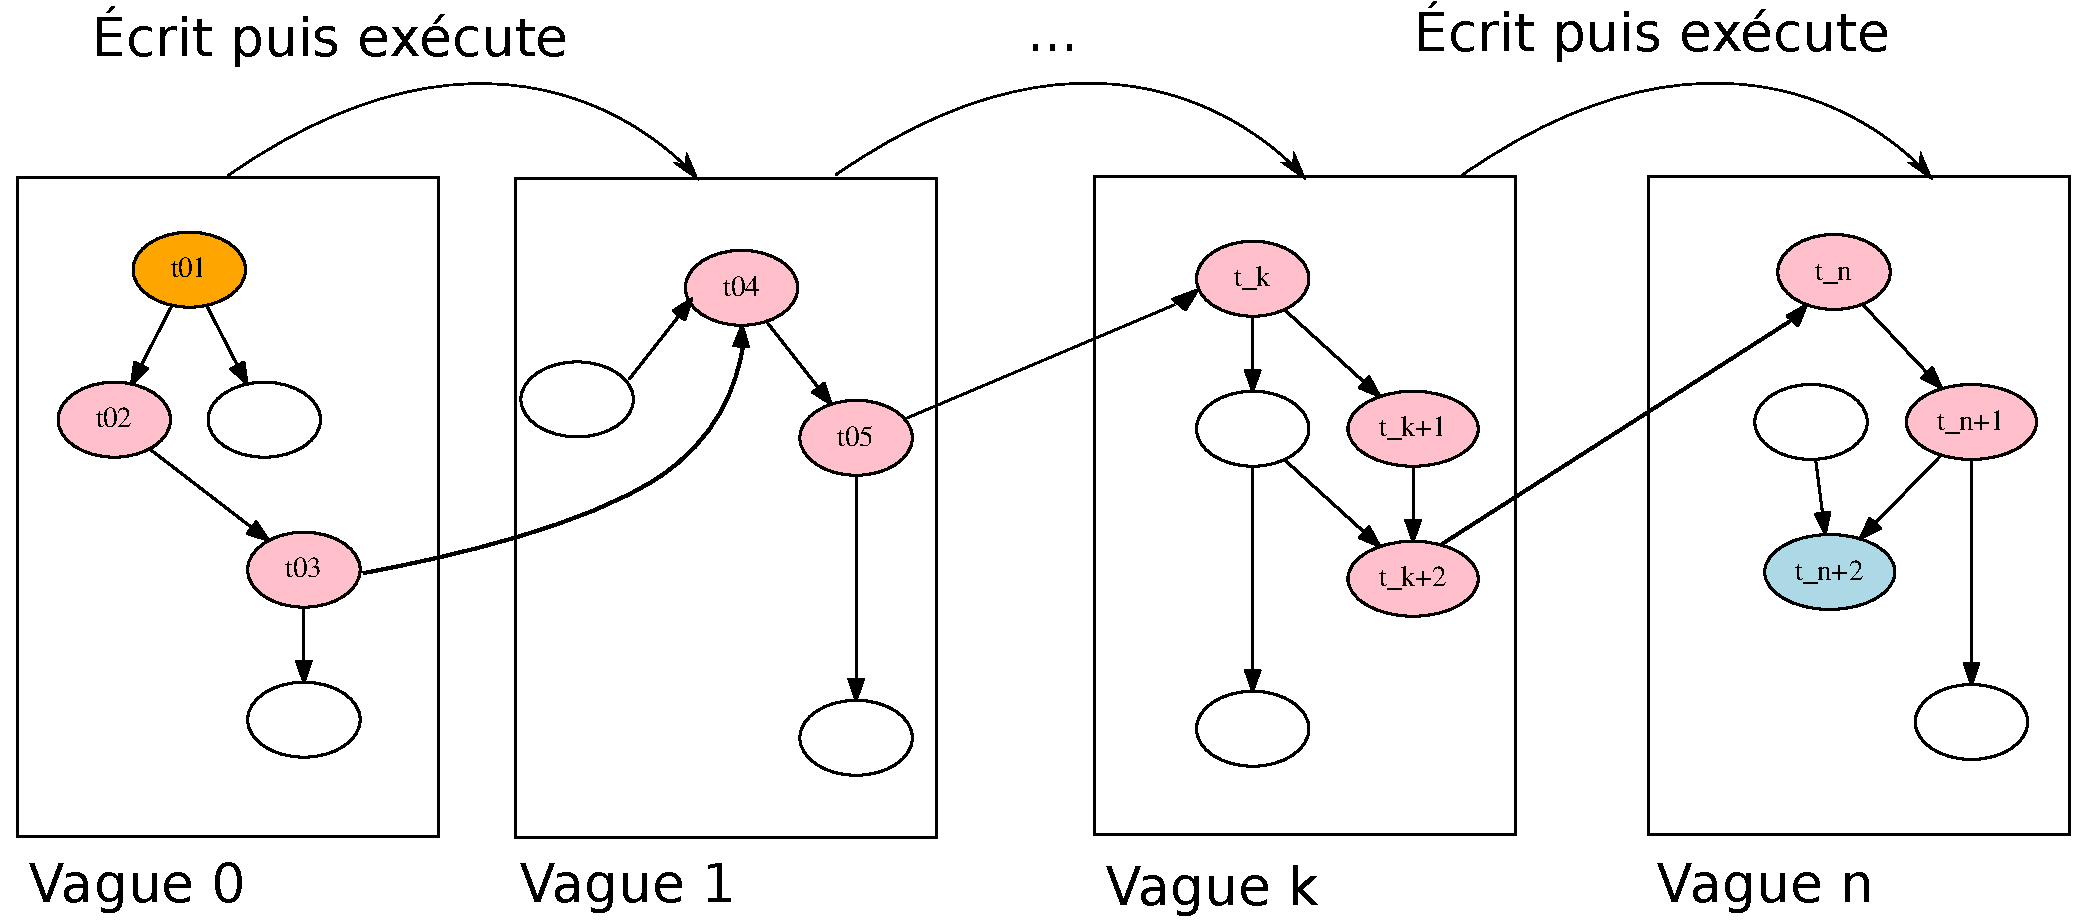
\includegraphics[width=1.0\textwidth]{supports/automodification/phases2_final.pdf}
 \caption{Vision informelle des vagues}
 \label{fig:vagues_visuel}
\end{figure}


\subsection{Revue de littérature}
La notion de vague présentée dans ce chapitre a été développée dans les thèse de Calvet \cite{Calvet2013} et Reynaud \cite{Reynaud2010}.
Elle est similaire à la notion de \emph{phase} présentée par Debray et Patel \cite{DP10} et utilisée pour automatiser la suppression de la protection d'un binaire.
En général la suppression des protections se fait à l'aide d'une analyse dynamique et d'une image de la mémoire à un instant donné au cours de l'exécution. C'est cette image mémoire qui sera considéré comme était le programme d'origine. La difficulté réside alors dans le choix de l'instant où prendre l'image mémoire.


\subsection{Trace, niveaux d'exécution et vagues}
Le programme exécuté a pour sources principales de données les registres et la mémoire constituée de la pile et du tas qui sont tous les deux adressables par des entiers. Une variable d'un programme est donc soit un registre du processeur soit une adresse mémoire, comme indiqué en définition \ref{def:variable}.
\begin{defi}
On définit l'ensemble $\BV$ des variables comme contenant un ensemble fini de registres $a\in\BA$ et un tableau de taille finie $\mathbb{T}=\textlbrackdbl 0,\ t\textrbrackdbl$.
\label{def:variable}
\end{defi}

En utilisant la sémantique concrète précédemment définie on est capable, à partir d'un ensemble de valeurs initiales pour les registres et la mémoire, d'exécuter un programme sur cette entrée.
Une trace d'exécution d'un programme est simplement l'enchaînement des instructions auxquelles l'exécution du programme a fait appel. Si on note $I_i$ une instruction dynamique, la trace d'exécution est $T=I_1, I_2, ..., I_n$ où $I_n$ est la dernière instruction du programme.

Nous définissons une instruction dynamique (définition \ref{def:ensembles_inst_dyn}) par son adresse, les adresses mémoires sur lesquelles elle est codée et l'instruction machine correspondant. Ces informations sont données par un désassemblage atomique d'une instruction à l'adresse mémoire spécifiée.
Afin de pouvoir séparer la trace d'exécution selon le moment où chaque instruction a été écrite, nous définissons aussi pour chaque instruction l'ensemble des variables sur lesquelles elle provoque une écriture. Cette information sera donnée par la sémantique concrète choisie \todo{sémantique}.

\begin{defi}
On note $D$ une instruction dynamique constituée des éléments suivants.
\begin{itemize}
 \item \da{D} l'adresse mémoire de l'instruction dynamique
 \item \dc{D} le segment des adresses mémoire sur lequel \di{D} est codée
 \item \di{D} l'instruction machine à l'adresse \da{D}
%  \item \dr{D_i} l'ensemble des variables sur lesquelles l'exécution de \di{D_i} provoque une lecture
 \item \dw{D} l'ensemble des variables sur lesquelles l'exécution de \di{D} provoque une écriture
\end{itemize}
\label{def:ensembles_inst_dyn}
\end{defi}

Nous avons donc, pour une trace d'exécution donnée, des vagues successives $1, 2, ..., n$. 
Au cours de l'exécution du programme on définit, pour chaque adresse en mémoire $m$, un niveau d'écriture $W^M[m]$.
correspondant à la dernière vague $k$ durant laquelle une instruction a modifié la valeur à l'adresse $m$.


Une instruction $D$ a un niveau d'exécution $X$, comme indiqué en définition \ref{def:write_exec_levels}.
Elle a également a un niveau d'écriture $W_D$ qui est le niveau d'écriture le plus élevé parmi les adresses sur lesquelles elle est codée : $W_D=max(W^M[a],\ a\in\ $\dc{D_i}$)$.


\begin{defi}
Nous définissons une trace d'exécution comme la donnée d'une suite $T=t_1, t_2, ..., t_n$ composée de triplets de la forme $t_i=(i, D_i, X_i)$ tels que
\begin{itemize}
 \item $D_i$ est la $i^{eme}$ instruction exécutée.
 \item Avant l'exécution de l'instruction $D_i$, le niveau d'exécution est \texttt{$X_{i-1}$}.
 \item Après l'exécution de l'instruction $D_i$, le niveau d'exécution est \texttt{$X_i$}.
\end{itemize}
\label{def:write_exec_levels}
\end{defi}

\begin{propri}
 Si le niveau d'exécution courant est $X$, le niveau d'exécution de l'instruction à exécuter $D_i$ est :\\
 $X=max(X, W_D+1)$ avec $W_D=max(W^M[a],\ a\in\ $\dc{D_i}$)$.\\
 Après l'exécution de $D_i$, les niveaux d'écriture dans la mémoire sont mis à jour de la manière suivante :\\
 $\forall a\in$ \dw{D_i}, $W^M[a]=X$.
\label{propri:niveau_exec}
\end{propri}

En pratique une instruction $D$ écrite par une instruction ayant pour niveau d'exécution $k$ puis directement exécutée aura pour niveau d'écriture $W_D=k$ et pour niveau d'exécution $X=k+1$. Ce comportement est formalisé par la propriété \ref{propri:niveau_exec}.

On définit alors formellement la vague $k$ selon la définition \ref{def:vagues} et l'algorithme \ref{algo:analyse_dyn_vagues} permet d'exécuter un programme dynamiquement avec la sémantique concrète choisie tout en déterminant les niveaux d'exécution de d'écriture au fur et à mesure de l'exécution. La sortie de l'algorithme \ref{algo:analyse_dyn_vagues} est la trace d'exécution et la liste des vagues reconstruites.
\\

Reprenons l'exemple du programme auto-modifiant de la figure \ref{fig:unevague_trace}.
La figure \ref{fig:unevague_trace} donne une trace d'exécution de ce programme en détaillant les informations sur chaque instruction dynamique ainsi que les niveaux d'écriture et d'exécution de chaque instruction.
Au départ toute la mémoire est dans son état d'origine et a pour niveau d'exécution 0. Lorsque l'instruction $D_0$ est exécutée, il n'y a pas eu d'auto-modification donc le niveau d'écriture est 0 et le niveau d'exécution est 1.
Les instructions $D_3$ et $D_4$ provoquent une auto-modification : les octets aux adresses \adr{0x8048091} et \adr{0x8048092} sont modifiés et leurs niveaux d'écriture deviennent donc le niveau d'exécution courant, soit 1.
Lorsque l'exécution atteint $D_5$, qui a été modifié, le niveau d'écriture est 1 donc le niveau d'exécution devient 2.
L'instruction suivante $D_6$ fixe la valeur de \edi\ à 2 puis les instructions suivantes provoquent l'affichage de \edi.

Cette trace d'exécution est donc composée de deux vagues : la vague initiale, $v_0$ composée de l'état de la mémoire avant l'exécution de la première instruction et la vague $v_1$ contenant l'état de la mémoire juste après l'exécution de $D_4$ et avant l'exécution de la première instruction modifiée $D_5$.




\begin{defi}
 Étant donné une trace d'exécution $T=t_1, ..., t_n$ avec $t_i=(i, D_i, X_i)$ et $k\in\{X_j, 1\leq i\leq n\}$, on appelle vague $k$ l'état de la mémoire juste après l'exécution de la dernière instruction ayant pour niveau d'exécution $k$.
 C'est à dire l'état de la mémoire juste après l'instruction $D_j$ avec $X_{j+1}>k$.
 \label{def:vagues}
\end{defi}

% \begin{algorithm}[H] %or another one check
% \caption{Mise à jour des niveaux d'exécution et d'écriture lors de l'exécution d'une instruction}
% \SetAlgoLined
% \KwIn{La mémoire, l'opérateur de niveau d'écriture, une instruction dynamique et le niveau d'exécution courant}
% \KwResult{L'opérateur de niveau d'écriture et le niveau d'exécution courant mis à jour}
% \SetKwProg{Fn}{}{}{}
% \SetKwFunction{FRecurs}{calculNiveau}
% \Fn(
% ){\FRecurs{M, $W^M$, D, X}}{
% $W_D \leftarrow\ max(W^M[a],\ a\in\ $\dc{D}$)$\\
% $X \leftarrow\ max(X,\ W_D+1)$ \\
% \For {$m\in\ $\dw{D}}{
%   $W^M[m]\leftarrow\ X$
% }
% \Return ($W^M$, X)
% }
% \label{algo:update_vagues}
% \end{algorithm}

\begin{algorithm}[H] %or another one check
\caption{Mise à jour du niveau d'exécution d'une instruction}
\SetAlgoLined
\KwIn{La mémoire, l'opérateur de niveau d'écriture, une instruction dynamique et le niveau d'exécution courant}
\KwResult{Le niveau d'exécution courant mis à jour}
\SetKwProg{Fn}{}{}{}
\SetKwFunction{FRecurs}{MAJExecution}
\Fn(
){\FRecurs{M, $W^M$, D, X}}{
$W_D \leftarrow\ max(W^M[a],\ a\in\ $\dc{D}$)$\\
$X \leftarrow\ max(X,\ W_D+1)$ \\
\Return X
}
\label{algo:update_exec_level}
\end{algorithm}

\begin{algorithm}[H] %or another one check
\caption{Mise à jour des niveaux d'écriture lors de l'exécution d'une instruction}
\SetAlgoLined
\KwIn{La mémoire, l'opérateur de niveau d'écriture, une instruction dynamique et le niveau d'exécution courant}
\KwResult{L'opérateur de niveau d'écriture mis à jour}
\SetKwProg{Fn}{}{}{}
\SetKwFunction{FRecurs}{MAJEcriture}
\Fn(
){\FRecurs{M, $W^M$, D, X}}{
\For {$m\in\ $\dw{D}}{
  $W^M[m]\leftarrow\ X$
}
\Return $W^M$
}
\label{algo:update_write_level}
\end{algorithm}

\begin{figure}
\begin{center}
\begin{tabular}[b]{|l|l|l|l|l|l|l|}
\hline
i & \da{D_i} & \dc{D_i} & \di{D_i} & \dw{D_i} & $W_i$ & $X_i$ \\
\hline
& 8048060  &  (...)         	        & Pile -> RWX &  & 0 & 1 \\ 
1 & 804807c  &  [804807c, 8048080]         &  mov    edi, 0x0 & edi & 0 & 1 \\
2 & 8048081  &  [8048081, 8048086]         &  mov    eax, 0x8048091 & eax & 0 & 1 \\
3 & 8048086  &  [8048086, 804808a]         &  mov    [eax], 0xeb & 0x8048091 & 0 & 1 \\
4 & 804808b  &  [804808b, 8048090]         &  mov    [eax+1], 0x7 & 0x8048092 & 0 & 1 \\
5 & 8048091  &  [8048091, 8048092]         &  jmp    80480a1 <edi3> &  & 1 & 2  \\
6 & 804809a  &  [804809a, 804809d]         &  mov    edi,0x2 & edi & 0 & 2\\
7 & 804809f  &  [804809f, 80480a0]         &  jmp    80480a8 <fin> &  & 0 & 2\\
 & 80480a8  &  (...)		        &  Affiche edi &  & 0 & 2\\
 & 80480c3  &  (...)		        &  Quitte &  & 0 & 2\\
\hline
\end{tabular}
\end{center}
\caption{Trace d'exécution du programme auto-modifiant de la figure \ref{fig:unevague_v0}}
\label{fig:unevague_trace}
\end{figure}

\todo[inline]{définir sem\_eval dans la sémantique}

\begin{algorithm}[H] %or another one check
\caption{Analyse dynamique avec calcul des vagues}
\SetAlgoLined
\KwIn{Les registres R et une mémoire M dans laquelle un programme a été chargé à son point d'entrée \texttt{ep}}
\KwResult{La trace des instructions dynamiques chacune associée à leur niveau d'exécution et les différentes vagues de la trace}
\SetKwProg{Fn}{}{}{}
\SetKwFunction{FRecurs}{analyseDynamique}
\Fn(
% \tcc*[h]{C : matrice des associations possibles, i : numéro du prochain sommet de P à associer, F : liste des couples d'associations déjà faites}
){\FRecurs{R, M, ep}}{
\For{$m\in M$}{
  $W^M[m]\leftarrow 0$\\
}
$X\leftarrow 1$\\
$X_{-1}\leftarrow 0$\\
$i\leftarrow 0$\\
$T\leftarrow \emptyset$\\
$vagues\leftarrow \emptyset$\\
$eip\leftarrow ep$\\
\While {la fin du programme n'est pas atteinte} {
$i\leftarrow i+1$\\
~\\
$D\leftarrow decode(eip, M)$\\
$X\leftarrow MAJExecution(M, W^M, D, X)$\\
\If {$X \ne X_{-1}$}{
  $vagues\leftarrow vagues\cup \{(X_{-1}, M)\}$
}
$X_{-1} \leftarrow X$\\
~\\
$(eip, R, M, D)\leftarrow sem\_eval(eip, R, M)$\\
$W^M\leftarrow MAJEcriture(M, W^M, D, X)$\\
$T\leftarrow T\cup\{(i, D_i, X)\}$\\
}
\Return T, vagues
}
\label{algo:analyse_dyn_vagues}
\end{algorithm}

\begin{rem}
 Étant donné la définition croissante des vagues, la même instruction $D$ peut-être exécutée non seulement plusieurs fois dans la même vague mais également être présente à des vagues différentes.
\end{rem}



\DontFrameThisInToc
\chapter{Analyse statique et hybride}
\todo[inline]{Objectifs : Code -> CFG + trouver tout le code possible}
\todo[inline]{Analyse statique : les possibilités et un exemple}

\paragraph{Découvrir exactement le code atteignable.}

\paragraph{Reconstruction du graphe de flot de contrôle.}

\section{Retour sur le chevauchement}
\paragraph{UPX}
UPX utilise le chevauchement pour optimiser la taille du binaire packé (figure \ref{fig:upx_obf_asm}).
La procédure de dé-package utilise un saut conditionnel pour séparer le contrôle de flot en deux blocs se chevauchants et finissant sur un bloc où ils se réalignent.
\todo{expliquer les deux branches, rapidement en quoi elles sont utiles}
\begin{figure}
\scriptsize
\begin{lstlisting}[language={[x86masm]Assembler}, escapechar=~]
    010059f0    89 f9            mov ecx, edi
,=< 010059f2    79 07            jns +9
|   010059f4    0f b7 07         movzx eax, word [edi]
|   010059f7    47               inc edi
|   010059f8    50               push eax
|   010059f9    47               inc edi
|   010059fa    b9 57 48 f2 ae   mov ecx, aef24857
`->   010059fb     57            push edi
      010059fc        48         dec eax
      010059fd           f2 ae   repne scasb
    010059ff    55               push ebp
\end{lstlisting}
% \end{framed}
\caption{Overlapping assembly in UPX.\label{fig:upx_obf_asm}}
\end{figure}
Le graphe de flot de contrôle pour ce chevauchement est donné en figure \ref{fig:upx_cfg}.

\begin{figure}
\begin{center}
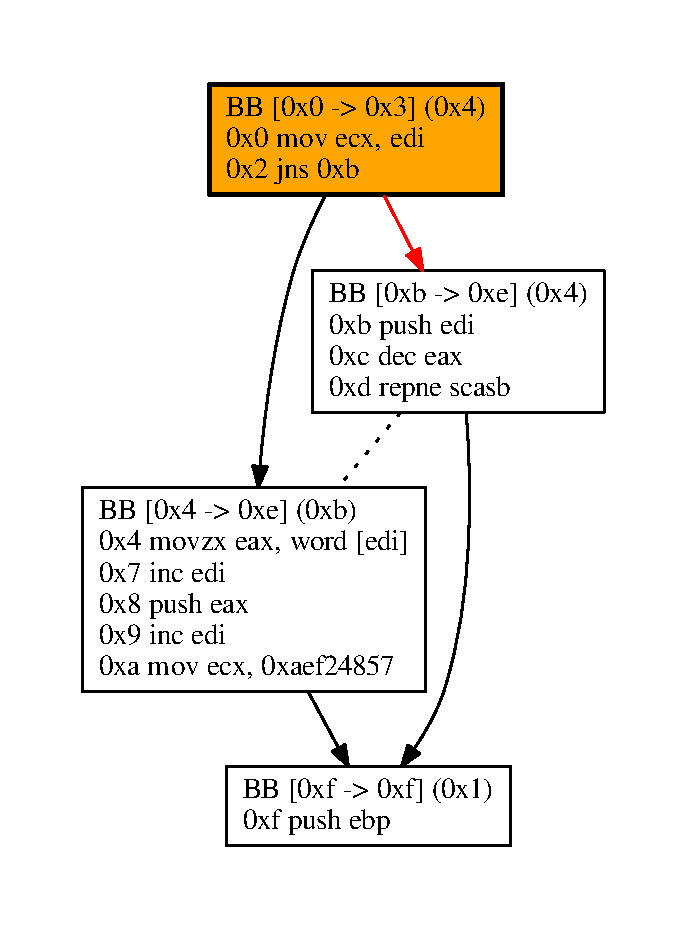
\includegraphics[width=0.4\textwidth]{supports/disasm/upx/upx.pdf}
\end{center}
\caption{Control flow graph for the UPX sample}
\label{fig:upx_cfg}
\end{figure}


\section{Sémantique pour un langage de type assembleur}
\todo[inline]{Comment elle gère l'auto-modification, les layers ?}

\paragraph{Structure des variables et de la mémoire.}

\begin{defi}
On définit les symboles $x\in\BX$ comme constitués de variables $v\in\BV$ et de pointeurs $p\in\BP$ vers des variables. $\BV$ contient un ensemble fini de registres $a\in\BA$ et un tableau de taille finie $\mathbb{T}=\textlbrackdbl 0,\ t\textrbrackdbl$. Les éléments de $\BP$ sont des pointeurs vers une variable : $\{[v],\ v\in \BV\}$.
\end{defi}


\paragraph{Instructions et programmes.}
\begin{defi}
Des labels $l\in\BL$ numérotent les instructions où $\BL$ est un sous-ensemble fini de $\BN$ contenant $\bot$. Les instructions sont de ce type : \\
$inst:=\ $\emph{$x\leftarrow g(x_1, ..., x_m)$ $|$ goto $x$ $|$ if $x$ then $goto\ x'$ $|$ end}\\
$prog:=\ $\emph{$l:inst\ |\ prog;\ l:inst$}\\
Les valeurs possibles pour les variables sont dans $\BN$.
\end{defi}
%On note $\PMN$ l'ensemble des parties de $\BN$ de taille inférieure ou égale à M $\in\BN$ en excluant l'ensemble vide (représenté par $\bot$).

\todo[inline]{Un opérateur D de désassemblage! D : l -> inst, taille}

\begin{defi}
$\sigma : \BV \rightarrow \Trs$ représente un store : à une variable du programme est associée soit une valeur, soit $\bot$ (valeur initiale) lorsqu'aucune valeur n'est connue, soit $\top$ lorsque toute valeur est possible ou que le maximum de valeurs M est atteint. Un ensemble de store est représenté par $\Sigma$ : $\Sigma\in\TTrs$.\\
\end{defi}

\todo[inline]{Exemple de programme}

\section{Interprêtation abstraite}
\todo[inline]{citer \cite{Kildall73}, \cite{CousotC77}, \cite{BHV11}}
\section{Value Set Analysis (VSA)}
\todo[inline]{Sémantique + interp abstraite pour VSA || explication informelle + limites ?}

\section{VSA pour les programmes auto-modifiants}

\todo[inline]{Relire pour comprendre}
\todo[inline]{Polir les notations avec D et adapter aussi pour VSA (?)}
\todo[inline]{Ajouter les sous-titres}

\section{Limites de VSA}

\section{Propagation}
\begin{defi}
Soit $\Sigma$ et $\Sigma'$ dans $\TTrs,\ \Sigma \vee \Sigma'=\Sigma \cup \Sigma'$ avec : 
\begin{itemize}
 \item Si $\exists\ v\in\BV,\ \sigma\in\Sigma\cup\Sigma',\ \sigma(v)=\top$ alors $\forall\sigma\in\Sigma\vee\Sigma',\ \sigma[v\leftarrow\top]$
 \item $\forall v\in\BV$, si $|\{\sigma(v), \sigma\in\Sigma\cup\Sigma'\}|>M$ alors $\forall\sigma\in\Sigma\vee\Sigma',\sigma[v\leftarrow\top]$
\end{itemize}
\end{defi}

\begin{defi}
 Définissons une extension $\sigma_X$ d'un store $\sigma : \BV \rightarrow \Trs$ à $\BX \rightarrow \Trs$. Soit $x\in\BX$.
 \begin{itemize}
  \item Si $x\in\BV$ : $\sigma_X(x)=\sigma(x)$
  \item Sinon, $x\in\BP$ : $x=\textlbrackdbl v\textrbrackdbl$ avec $v\in\BV$.
  \begin{itemize}
   \item Si $\sigma(v)=\top$ alors $\sigma_X(x)=\top$
   \item Si $\sigma(v)=\bot$ alors $\sigma_X(x)=\bot$
   \item Si $\sigma(v)\in\BN$ et $\sigma(v)>t$ alors $\sigma_X(x)=\bot$
   \item Sinon $\sigma(v)\in\BN$ et $\sigma(v)\in\BT$, alors $\sigma_X(x)=\sigma(\sigma(v))$.
  \end{itemize}

 \end{itemize}
\end{defi}

\begin{defi}
Soit $g:\BN^m  \rightarrow \BN$ (avec $m\in\BN$) une fonction totale sur son domaine.
Notons V l'évaluation de $g(x_1, ..., x_m)$ :
$V=
\left\{
  \begin{array}{ll}
	  \bot &$ si $\exists i / \sigma_X(x_i)=\bot
	\\\top &$ si $\exists i / \sigma_X(x_i)=\top
	\\ g(\sigma_X(x_1), ..., \sigma_X(x_m)) &$ sinon.$
  \end{array}
\right.
$\\
\end{defi}

\begin{defi}
Soit $g:\BN^m  \rightarrow \BN$ (avec $m\in\BN$) une fonction totale sur son domaine, on définit $f(l,\sigma)$ :
\begin{itemize}
\item Si l'instruction $l$ est de type $x\leftarrow g(x_1, ..., x_m)$ avec $x_1, x_2, ..., x_m$ dans $\BX$ alors : \\
$f(l, \sigma) = \sigma$ modifié comme suit : $
\left\{
  \begin{array}{ll}
	  \sigma\leftarrow\sigma[x\leftarrow V] &$ si $x\in\BV
	\\$non modifié$ &$ si $\sigma_X(x)=\bot
	\\\forall v\in\BV,\ \sigma(v)=V &$ si $\sigma_X(x)=\top
	\\\sigma\leftarrow\sigma[\sigma_X(x)\leftarrow V] &$ sinon ($\sigma_X(x)\in\BN$ et $\sigma_X(x)\in\BT)
  \end{array}
\right.
$\\

\item Sinon $f(l, \sigma)=\sigma$.
\end{itemize}
\end{defi}

\section{Analyse statique progressive et bornée}
On définit, pour un label $l\in\BN$ et un store $\sigma$, l'ensemble des labels successeurs $I(l, \sigma)$ comme suit.
\begin{itemize}
 \item Si $l : x\leftarrow g(x_1, ..., x_m)$ alors $I(l, \sigma)=\{l+1\}$

 \item Si $l : goto\ x$ alors
 \begin{itemize}
  \item Si $\sigma_X(x)=\bot$ alors $I(l, \sigma)=\emptyset$
  \item Si $\sigma_X(x)\in\BN$% $I(l, \sigma)=\sigma(v)$
  \begin{itemize}
   \item Si $\sigma_X(x)\notin\BL$, $I(l, \sigma)=\emptyset$
   \item Sinon, $\sigma_X(x)\in\BL$ et $I(l, \sigma)=\{\sigma(x)\}$
  \end{itemize}
  \item Sinon, $\sigma_X(x)=\top$ et $I(l, \sigma)=\BL$
 \end{itemize}
 \item Si $l : if \ b\ then\ goto\ x$ alors
 \begin{itemize}
  \item Si $\sigma_X(b)=1$ alors $I(l, \sigma)=I(l:goto\ x, \sigma)$
  \item Si $\sigma_X(b)\in\BN\cup\{\bot\}$ alors $I(l, \sigma)=I(l:goto\ l+1, \sigma)$
  \item Sinon, $\sigma_X(b)=\top$ et $I(l, \sigma)=I(l:goto\ x, \sigma)\cup I(l:goto\ l+1, \sigma)$
 \end{itemize}
 \item Si $l : end$ alors $I(l, \sigma)=\emptyset$
 \item Si $l\notin\BL$ alors $I(l, \sigma)=\emptyset$
%  \item Si $l=\bot$ alors $I(l, \sigma)=\emptyset$
\end{itemize}

 On définit, pour un ensemble de stores, ses labels successeurs par $I(l, \Sigma)=\bigcup_{\sigma\in\Sigma}I(l,\sigma)$.\\


% \begin{algo}
Soit l'algorithme suivant. On note $\Sigma_l$ l'approximation courante à l'instruction de label $l$, et $E_l$ indique si l'instruction a déjà été explorée.\\
On conserve une liste de labels à explorer sous la forme de couples $(l,\Sigma)$ où $l$ est un label et $\Sigma$ un ensemble de stores.\\
Notons $\sigma_{init}$ le store vide défini par : $\forall v \in \mathbb{V}, \sigma_{init}(v)=\bot$.
On initialise L à partir des points d'entrée : pour chaque point d'entrée de label $l$, L contient $(l, \{\si\})$.
\\
\\
$\begin{array}{ll}
 Init & \forall i \in \BL$, $\Sigma_i\leftarrow\emptyset$, $E_i\leftarrow false\\
  & L\leftarrow e$ (points d'entrée, par exemple (1, $\{\si\}$))$\\
Boucle & $Si $L=\emptyset$, arrêt$\\
Selection & $Soit (l, $\Sigma)\in L$, $L\leftarrow L-{(l, \Sigma)}\\
Avancer & $Si $\Sigma\leq\Sigma_l$ et $E_l=true$ alors aller à Boucle$\\
  & $Sinon $\Sigma'_l\leftarrow\Sigma_l\vee\Sigma\\
  & \ \ \ \ \ \ \ \ \Sigma^{diff}\leftarrow\Sigma'_l-\Sigma_l\\
  & \ \ \ \ \ \ \ \ \Sigma_l\leftarrow\Sigma'_l\\
  & \ \ \ \ \ \ \ \ \forall s\in I(l,\Sigma^{diff}), \Sigma^+_s=\{f(I,\ \sigma),\ \sigma\in\Sigma^{diff},\ s\in I(l,\sigma)\}\\
  & \ \ \ \ \ \ \ \ L\leftarrow L\cup \bigcup_{s}(s,\Sigma^+_s)\\
  & \ \ \ \ \ \ \ \ E_l=true\\
  & \ \ \ \ \ \ \ $ aller à Boucle$\\
\end{array}$
\\
\\\\
Lors de l'étape Avancer, l'idée est simplement de séparer les stores selon leurs successeurs et de n'ajouter à L que ceux qui n'y ont jamais été ajoutés (les autres ont déjà été propagés).\\
En sortie de l'algorithme, on a, pour chaque instruction $l$, une sur-approximation $\Sigma_l$ de l'ensemble des stores possibles en entrée de l'instruction.
\\

\section{Exemples}
\subsection{Boucle simple}

\begin{tabbing}
1\ \  \=: a=3\\
2 \>: a=a+1\\
3 \>: if $a\leq 4$ goto 2\\
4 \>: end
\end{tabbing}

Appliquons l'analyse pour M=2.

\begin{tabbing}
Init. L=(1, $\{\si\}$).\\
Sélection de (1,\= $\{\si\}$).\\
Avancer. \> $E_1=false$ donc $\Sigma_1=\Sigma_1\vee\{\si\}=\{\si\}=\Sigma^{diff}$\\
\> $I(1,\Sigma^{diff})=\{2\}$, $\Sigma^+_2=\{[a\leftarrow 3]\}$.\\
\> $L=(2,\{[a\leftarrow 3]\})$\\
\> $E_1=true$\\

Sélection de $(2,\{[a\leftarrow 3]\})$.\\
Avancer. \> $E_2=false$ donc $\Sigma_2=\Sigma_2\vee\{[a\leftarrow 3]\}$=$\{[a\leftarrow 3]\}=\Sigma^{diff}$.\\
\> $I(2,\Sigma^{diff})=\{3\}$, $\Sigma^+_3=\{[a\leftarrow 4]\}$.\\
\> $L=\{[a\leftarrow 4]\}$\\
\> $E_2=true$\\

Sélection de $(3,\{[a\leftarrow 4]\})$.\\
Avancer. \> $E_3=false$ donc $\Sigma_3=\Sigma_3\vee\{[a\leftarrow 4]\}$=$\{[a\leftarrow 4]\}=\Sigma^{diff}$.\\
\> $I(3,\Sigma^{diff})=\{2\}$ car $[a\leftarrow 4](a)=4$, $\Sigma^+_2=\{[a\leftarrow 4]\}$.\\
\> $L=(2,\{[a\leftarrow 4]\})$\\
\> $E_3=true$\\

Sélection de $(2,\{[a\leftarrow 4]\})$.\\
Avancer. \> $\Sigma$ et $\Sigma_2$ ne sont pas comparables donc $\Sigma_2=\Sigma_2\vee\{[a\leftarrow 4]\}$=$\{[a\leftarrow 3],[a\leftarrow 4]\}$ et $\Sigma^{diff}=[a\leftarrow 4].$\\
\> $I(2,\Sigma^{diff})=\{3\}$, $\Sigma^+_3=\{[a\leftarrow 5]\}$.\\
\> $L=(3,\{[a\leftarrow 5]\}$)\\

Sélection de $(3,\{[a\leftarrow 5]\})$.\\
Avancer. \> $\Sigma$ et $\Sigma_3$ ne sont pas comparables donc $\Sigma_3=\Sigma_3\vee\{[a\leftarrow 5]\}$=$\{[a\leftarrow 4],[a\leftarrow 5]\}$ et $\Sigma^{diff}=[a\leftarrow 5].$\\
\> $[a\leftarrow 5](a)=5>4$ donc $I(3,\Sigma^{diff})=\{4\}$, $\Sigma^+_4=\{[a\leftarrow 5]\}$.\\
\> $L=(4,\{[a\leftarrow 5]\})$\\

Sélection de $(4,\{[a\leftarrow 5]\})$.\\
Avancer. \> $\Sigma$ et $\Sigma_4$ ne sont pas comparables donc $\Sigma_3=\Sigma_3\vee\{[a\leftarrow 5]\}$=$\{[a\leftarrow 5]\}$\\
\> $I(4,\Sigma^{diff})=\emptyset$.\\
\> $L=\emptyset$\\
Arrêt sur Boucle.

\end{tabbing}

On peut consigner ces résultats dans un tableau. Les colonnes $l$ et $\Sigma$ suivent l'exécution de l'algorithme en montrant le choix fait à l'étape Sélection. $\Sigma^{in}_l$ est le $\Sigma_l$ au moment de sa première lecture dans l'étape Avancer, $\Sigma^{out}_l$ celui au moment la sortie de l'étape Avancer, et L l'ensemble L à la sortie de l'étape Avancer.
Il est à noter que $\Sigma_l$ correspond toujours à l'état de l'approximation \emph{avant} l'interprêtation de l'instruction au label $l$.\\ 

\begin{tabular}{|l|l|l|l|l|l|}
 \hline 
 l & $\Sigma$ & $\Sigma^{in}_i$ & $\Sigma^{out}_l$ & $\Sigma^{diff}$ & L\\
 \hline
 Init & - & - & - & - & (1, $\{\si\}$)\\
 1 & $\{\si\}$ & $\emptyset$ & $\{\si\}$ & $\{\si\}$ & $(2,\{[a\leftarrow 3]\})$\\
 2 & $\{[a\leftarrow 3]\}$ & $\emptyset$ & $\{[a\leftarrow 3]\}$ &  $\{[a\leftarrow 3]\}$ &  $(3,\{[a\leftarrow 4]\})$\\
 3 & $\{[a\leftarrow 4]\}$ & $\emptyset$ & $\{[a\leftarrow 4]\}$ &  $\{[a\leftarrow 4]\}$ &  $(2,\{[a\leftarrow 4]\})$\\
 2 & $\{[a\leftarrow 4]\}$ & $\{[a\leftarrow 3]\}$ & $\{[a\leftarrow 3]\, [a\leftarrow 4]\}$ &  $\{[a\leftarrow 4]\}$ &  $(3,\{[a\leftarrow 5]\})$\\
 3 & $\{[a\leftarrow 5]\}$ & $\{[a\leftarrow 4]\}$ & $\{[a\leftarrow 4],[a\leftarrow 5]\}$ &  $\{[a\leftarrow 5]\}$ &  $(4,\{[a\leftarrow 5]\})$\\
 4 & $\{[a\leftarrow 5]\}$ & $\emptyset$ & $\{[a\leftarrow 5]\}$ &  $\{[a\leftarrow 5]\}$ &  $\emptyset$\\
 \hline
\end{tabular}

\section{Preuve de terminaison}
\subsection{Propriétés et corollaires}
\begin{defi}
 Soit $\leq$ l'ordre partiel sur $\Trs$ défini par :
 \begin{itemize}
  \item $\forall A\in \Trs, A \leq \top$
  \item $\forall A\in \Trs, A \leq A$
%  \item $\forall A\in \Trs, \bot \leq A$
%   \item $\forall A, B$ dans $\BN, \leq$ est l'ordre sur les entiers naturels
 \end{itemize}
\end{defi}

\begin{defi}
 Soit $\Sigma,\ \Sigma'\ dans\ \TTrs$, $\Sigma\leq\Sigma'$ si et seulement si $\forall\sigma\in\Sigma,\exists\sigma'\in\Sigma', \sigma\leq\sigma'$.
\end{defi}

\begin{defi}
 On définit la valuation d'une variable dans un ensemble de store comme suit :\\
 $V(\Sigma,v)=\left\{
  \begin{array}{ll}
	  M+1 &$ si $\exists \sigma\in\Sigma,\ \sigma(v)=\top\\
	|\{\sigma(v),\ \sigma\in\Sigma\}| &$ sinon$
  \end{array}
\right.$
\end{defi}

\begin{defi}
 On définit la valuation d'un ensemble de stores par : $V(\Sigma)=\sum_{v\in\BV} V(\Sigma,v)$.
\end{defi}

\begin{defi}
 Un ensemble de store $\Sigma$ est bien formé s'il vérifie les deux conditions suivantes :
 \begin{itemize}
  \item $\forall v\in\BV$, si $\exists \sigma\in\Sigma,\ \sigma(v)=\top$ alors $\forall\sigma\in\Sigma,\sigma(v)=\top$
  \item $\forall v\in\BV,\ |\{\sigma(v),\ \sigma\in\Sigma\}|\leq M$
 \end{itemize}
\end{defi}

\begin{prop}
 $\vee$ est commutatif et associatif. \qed
\end{prop}

\begin{prop}
Quels que soient $\Sigma$ et $\Sigma'$ dans $\TTrs$, $\Sigma\vee\Sigma'$ est bien formé. \qed
\end{prop}

\begin{prop}
\label{propSup}
Quels que soient $\Sigma$ et $\Sigma'$ dans $\TTrs$, $\Sigma\leq\Sigma\vee\Sigma'$. \qed
\end{prop}

\begin{prop}
\label{propCard}
 $\forall\ \Sigma,\ \Sigma'$ dans $\TTrs$ bien formés,$\ \Sigma \leq \Sigma'\Rightarrow V(\Sigma) \leq V(\Sigma')$ et $\forall v\in\BV,\ V(\Sigma,v) \leq V(\Sigma',v)$. \qed
\end{prop}

\begin{pr}
 Soit $v\in\BV$, on montre que $V(\Sigma,v)\leq V(\Sigma',v)$. Par cas.
 \begin{itemize}
  \item Si $\exists \sigma\in\Sigma,\ \sigma(v)=\top$ alors $\exists \sigma'\in\Sigma',\ \sigma'(v)\geq\sigma(v)=\top$ donc $\sigma'(v)=\top$ et $V(\Sigma',v)=V(\Sigma,v)=M+1$.
  \item Sinon, notons $(\sigma_1,...,\sigma_m)$ dans $\Sigma$ tels que $V(\Sigma,v)=m$. En particulier toutes les valeurs $\sigma_i(v)$ sont dans $\BN\cup\{\bot\}$ et deux à deux disjointes. $\Sigma\leq\Sigma'$ donc $\exists (\sigma'_1,...,\sigma'_m)$ tel que $\forall i,\ \sigma_i\leq\sigma'_i$ donc $\sigma_i(v)\leq\sigma'_i(v)$. Par définition de l'ordre partiel, soit $\exists i,\ \sigma'_i(v)=\top$ et $M+1=V(\Sigma',v)\geq V(\Sigma,v)$ car $V(\Sigma,v)\leq M$, soit $\forall i, \sigma'_i(v)=\sigma_i(v)$ et $\{\sigma(v),\ \sigma\in\Sigma\}\subset\{\sigma'(v),\ \sigma'\in\Sigma'\}$ donc $V(\Sigma,v)\leq V(\Sigma',v)$.
 \end{itemize}
\end{pr}


\begin{prop}
\label{propCard2}
 $\forall\ \Sigma,\ \Sigma'$ dans $\TTrs$ bien formés,$\ \Sigma < \Sigma\vee\Sigma'$ $\Rightarrow$ 
 $\left\{
  \begin{array}{ll}
	  V(\Sigma) < V(\Sigma\vee\Sigma')
	\\ou
	\\Card\ \Sigma < Card\ \Sigma\vee\Sigma'
  \end{array}
\right.$
\end{prop}

\begin{pr}
Notons $\Sigma''=\Sigma\vee\Sigma'$.\\
Par définition de $\vee$, deux cas sont possibles :
\begin{itemize}
 \item $\Sigma''\neq\Sigma\cup\Sigma'$ :\\
       Dans ce cas, un $\top$ a été ajouté comme valeur. Soit $v\in\BV$ tel que $\exists (\sigma,\sigma'')\in\Sigma\times\Sigma'', \sigma(v)\neq\top$ et $\sigma''(v)=\top$.\\
       Comme $\Sigma$ et $\Sigma''$ sont bien formés, $\forall (\sigma,\sigma'')\in\Sigma\times\Sigma'', \sigma(v)\neq\top$ et $\sigma''(v)=\top$.\\
       On en déduit que $V(\Sigma,v)\leq M$ et $V(\Sigma'',v)=M+1$.\\
       De plus $\Sigma\leq \Sigma''$ donc $\forall v\in\BV,\ V(\Sigma,v)\leq V(\Sigma'',v)$.\\
       Donc $V(\Sigma)<V(\Sigma'')$.
 \item $\Sigma''=\Sigma\cup\Sigma'$ :\\
       Comme $\Sigma''\neq\Sigma$, $Card\ \Sigma<Card\ \Sigma''$.
\end{itemize}

\end{pr}

\begin{cor}
\label{corCard}
 $\forall\ \Sigma,\ \Sigma'$ bien formés, si $V(\Sigma) = V(\Sigma\vee\Sigma')$ alors $Card\ \Sigma \leq Card\ \Sigma\vee\Sigma'$ 
\end{cor}
\begin{pr}
 Si $\Sigma=\Sigma\vee\Sigma'$ alors $Card\ \Sigma = Card\ \Sigma\vee\Sigma'$.\\
 Sinon $\Sigma<\Sigma\vee\Sigma'$, et comme $V(\Sigma) = V(\Sigma\vee\Sigma')$, $Card\ \Sigma < Card\ \Sigma\vee\Sigma'$.
\end{pr}

\begin{prop}
 La valuation et le cardinal sont bornés pour des stores bien formés :
 \begin{itemize}
  \item $\exists C\in\BN, \forall\ \Sigma\in\TTrs$ bien formé, $V(\Sigma)\leq C$.
  \item $\exists C\in\BN, \forall\ \Sigma\in\TTrs$ bien formé, $Card\ Sigma\leq C$.
 \end{itemize}
\end{prop}

\begin{pr}
 $V(\Sigma)=\sum_{v\in\BV} V(\Sigma,v)$ avec $\forall v\in\BV,\ V(\Sigma,v)\leq M+1$ donc $V(\Sigma)\leq (M+1)*Card\ \BV$.\\
 Quel que soit $v\in\BV$, il y a au plus M+1 valeurs pour $\sigma(v),$ où $\sigma\in\Sigma$ et $\sigma$ est défini par $(\sigma(v_1), \sigma(v_2)..., \sigma(v_n))$ avec $n$ le nombre de variables dans $\BV$.
 On en déduit que $Card\ \Sigma\leq (M+1)^{Card\ \BV}$. 
\end{pr}

\subsection{Terminaison}
On cherche à prouver que, passé un certains nombre d'itérations dans la boucle, il n'y a plus d'éléments à ajouter à L. Donc, puisqu'à chaque itération un élément en est retiré (étape Sélection), il arrivera que $L=\emptyset$ et donc l'algorithme se terminera (test de Boucle).\\

On numérote les passages dans la boucle (à l'étape Avancer) avec $k\in\mathbb{N}$ et $\Sigma_{l, k}$ est le $\Sigma_l$ calculé à la $k^{\text{ième}}$ itération. Dans le cas où $\Sigma_l$ n'est pas modifié à l'étape Avancer ($l$ n'est pas sélectionné ou si $\Sigma\leq\Sigma_l$), on prend $\Sigma_{l, k}=\Sigma_{l, k-1}$.

En vertu de la propriété \ref{propSup}, quels que soient i, k dans $\BN$, $\Sigma_{i, k}\leq\Sigma_{i, k+1}$, donc d'après la propriété \ref{propCard}, la suite $(V(\Sigma_{i,k}))_k$ est croissante. Elle est de plus bornée donc stationnaire à partir de $C\in\BN$. En vertu du corollaire \ref{corCard}, à partir de $k\geq C$ la suite $(Card\ \Sigma_{i,k})_{k\geq C}$ est croissante. Elle est également bornée donc stationnaire à partir de $C'\in\BN$.


Supposons que la suite $(\Sigma_{i,k})_k$ n'est pas stationnaire. Il existe alors $C''\in\BN$ avec $C''\geq C'$ vérifiant $\Sigma_{i,C''+1}>\Sigma_{i,C''}$. On en déduit, d'après la proposition \ref{propCard2}, que $Card\ \Sigma_{i,C''+1}>Card\ \Sigma_{i,C''}$, ce qui est contradictoire. Chaque suite $(\Sigma_{i,k})_k$ est donc stationnaire.
\\

Il y a un nombre fini de variables et d'instructions dans le programme donc $\exists K\in\BN, \forall i\in\BL, \forall k\in\BN, \Sigma_{i,k+K}=\Sigma_{i,K}$.
On en déduit qu'à partir de l'itération K de l'algorithme, on n'ajoute plus d'éléments à L. À ce point L est donc fini, de taille $|L|$ et sera vidé en un nombre maximum $|L|$ d'itérations supplémentaires.
L'algorithme termine.

% \end{algo}

\section{Correction de l'algorithme}
Soit t une exécution du programme : $t=(t_1,\ t_2..., t_p)$ avec $t_i=(l_i, \Theta_i)$, $t_1\longrightarrow t_2\longrightarrow ...\longrightarrow t_p$ et $l_p = \bot$.\\
On cherche à montrer que, à chaque instruction, le store calculé sémantiquement est bien un des stores trouvé par l'analyse statique, aux problèmes de surcapacité ($\top$) près, c'est à dire : $\forall n, \{\Theta_n\}\leq\Sigma_{l_n}$.


\subsection{Preuve par récurrence}
Soit $n\in \BN$, supposons que $l_n$ n'est pas $\bot$, que $l_n$ est atteint au moins une fois par l'analyse statique et que $\{\Theta_n\}\leq\Sigma_{l_n}$. On cherche à montrer que, dans le cas où $l_{n+1}$ n'est pas $\bot$, $l_{n+1}$ est atteint par l'analyse statique et que $\{\Theta_{n+1}\}\leq\Sigma_{l_{n+1}}$.
\subsection{Initialisation}
A l'initialisation, l'analyse statique débute avec $l_0$ comme point d'entrée et $\forall v\in\BV, \Theta_0(v)=\bot$ donc $\{\Theta_0\}\leq\Sigma_{l_0}$.
\subsection{Récurrence}
Soit k le dernier indice (dans la boucle de déroulement de l'algorithme) auquel $\Sigma_{{l_n},k}$ est modifié. k existe car $l_n$ est atteint par l'analyse statique et $\Sigma_{l_n}$ est modifié au moins une fois s'il est atteint (variables $E_i$). On règle chaque cas (selon l'instruction $l_n$) séparément en se plaçant à la $k^e$ itération de l'algorithme.\\
Notons $\Sigma^{-}_{l_n}=\Sigma_{{l_n},k-1}$, sachant que $\Sigma_{l_n}=\Sigma_{{l_n},k}$.

\begin{itemize}
 \item $l_n : a\leftarrow g(b_1, ..., b_m)$ :\\
 Sémantiquement, $t_{n+1}=(l_n+1, \Theta_n[a\leftarrow g(\Theta_n(b_1),\ \Theta_n(b_2)...,\ \Theta_n(b_m))])$ \\où $t_{n+1}=(l_n+1, \Theta_n[v\leftarrow\bot])$.\\
 Comme $\{\Theta_n\}\leq\Sigma_{l_n}$, $\exists\sigma\in\Sigma_{l_n}$ tel que $\forall v\in\BV,\ \Theta_n(v)\leq\sigma(v)$. Soit $\sigma$ un store vérifiant cette propriété.
 Notons $\sigma'$ le store résultant de l'opération d'union et $\sigma''$ le store finalement ajouté à L (après interprêtation de l'action de g sur a).\\
 Dans le déroulement de l'algorithme, à l'étape Avancer pour $\Sigma^-_{{l_n},k}$, comme $I(l_n,\sigma'')=\{l_n+1\}$, $(l_n+1, \Sigma_1)$ est ajouté à L avec $\sigma''\in\Sigma_1$.\\
 Dans une étape Sélection suivante, $(l_n+1, \Sigma_1)$ est donc sélectionné, on en conclut que le label $l_{n+1}=l_n+1$ est atteint par l'analyse statique.\\
 On veut montrer que le store $\sigma''$ résultant de l'analyse statique vérifie : $\forall v\in\BV,\ \Theta_{n+1}(v)\leq\sigma''(v)$.
 Seule la variable a est modifiée sémantiquement. Dans l'analyse statique d'autres variables peuvent être modifiées, mais uniquement lors de l'union des deux ensembles de stores et dans ce cas la variable v modifiée devient $\sigma''(v)=\top$, vérifiant systématiquement la propriété $\Theta_{n+1}(v)\leq\sigma''(v)$.\\
 Traitons le cas où l'opération d'union résulte en l'ajout d'un $b_i$ pour lequel $\sigma'(b_i)=\top$. Dans ce cas $\sigma''(a)=\top$ et $\Theta_{n+1}(a)\leq\top$.\\
 Vérifions à présent le cas contraire où $\sigma=\sigma'$, il y a à nouveau trois possibilités.
 \begin{itemize}
  \item Si $\exists i, \sigma(b_i)=\bot$, dans ce cas, comme $\Theta_n(b_i)\leq\sigma(b_i)$, on a : $\Theta_n(b_i)=\bot$. Donc $\Theta_{n+1}(a)=\bot=\sigma''(a)$.
  \item Si $\exists i, \sigma(b_i)=\top$, dans ce cas $\sigma''(a)=\top$ et $\Theta_{n+1}(a)\leq\top$.
  \item Sinon $\forall i,\sigma(b_i)\in\PN$. Si $\exists i,\Theta_n(b_i)=\bot$ alors $\Theta_{n+1}(a)=\bot\leq\sigma''(a)$. Dans le cas contraire, comme $\forall i,\Theta_n(b_i)\leq\sigma(b_i)$, on en déduit que $\forall i,\Theta_n(b_i)\in\PN$ et donc que $\forall i,\Theta_n(b_i)=\sigma(b_i)$. Donc $\Theta_{n+1}(a)=\sigma''(a)$.
 \end{itemize}
 On a démontré qu'on ajoute à L un élément $(l_{n+1}, \Sigma_1)$ avec $\sigma''\in\Sigma_1$ et $\Theta_{n+1}\leq\sigma''$. Dans une étape suivante, $(l_{n+1}, \Sigma_1)$ sera sélectionné et, après réunion, on aura bien $\{\Theta_{n+1}\}\leq\{\sigma''\}\leq\Sigma_{l_{n+1}}$ car $\sigma''\in\Sigma_1$ donc $\{\sigma''\}\leq\Sigma_1$ et $\Sigma_1\leq\Sigma_1\vee\Sigma^-_{l_{n+1}}=\Sigma_{l_{n+1}}$ d'après la propriété \ref{propSup}.
 \item $l_n : goto\ l$ :\\
  $t_{n+1}=(l, \Theta_n)$ et dans l'analyse, à l'étape Avancer, $(l, \Sigma_{{l_n},k})$ est ajouté à L. Donc dans une étape suivante, le label $l$ est atteint avec $\{\Theta_{n+1}\}=\{\Theta_n\}\leq\Sigma_{l_n}\leq\Sigma_{l_{n+1}}$.
 \item $l_n : if\ b\ then\ goto\ l$ :\\
  Comme $\{\Theta_n\}\leq\Sigma_{l_n}$, $\exists\sigma\in\Sigma_{l_n}$ tel que $\forall v\in\BV,\ \Theta_n(v)\leq\sigma(v)$. Soit $\sigma$ un store vérifiant cette propriété.
 % Dans l'analyse, à l'étape avancer, $(l, \Sigma_{{l_n},k})\cup(l_n+1, \Sigma_{{l_n},k})$ est ajouté à L.
  \begin{itemize}
   \item Si $\sigma(b)$ est $1$ :\\
   $\Theta(b)\leq\sigma(b)$ donc $\Theta(b)=1$. $(l, \Sigma_{l_n})$ est ajouté à L et $l_{n+1}=l$. $l_{n+1}$ est donc atteint par l'analyse statique et $\Sigma_{l_n}$ comme $\Theta_n$ n'ont pas été modifiés donc $\{\Theta_{n+1}\}\leq\Sigma_{l_{n+1}}$.
  
   \item Si $\sigma(b)$ est soit un entier différent de 1, soit $\bot$ :\\
   $\Theta(b)\leq\sigma(b)$ donc $\Theta(b)=\sigma(b)$. $(l_n+1, \Sigma_{l_n})$ est ajouté à L et $l_{n+1}=l_n+1$. $l_{n+1}$ est donc atteint par l'analyse statique et $\Sigma_{l_n}$ comme $\Theta_n$ n'ont pas été modifiés donc $\{\Theta_{n+1}\}\leq\Sigma_{l_{n+1}}$.
  
   \item Sinon $\sigma(b)$ est $\top$ :\\
   Dans ce cas $(l, \Sigma_{l_n})\cup(l_n+1, \Sigma_{l_n})$ est ajouté à L alors que $l_{n+1}$ est soit $l$, soit $l_n+1$. $l_{n+1}$ est donc atteint par l'analyse statique et $\Sigma_{l_n}$ comme $\Theta_n$ n'ont pas été modifiés donc $\{\Theta_{n+1}\}\leq\Sigma_{l_{n+1}}$.
  \end{itemize}
 \item $l_n : end$ :\\
   Les stores ne sont pas modifiés et le label suivant $l_{n+1}=\bot$ est atteint avec $I(l_n,\sigma)=\bot$ ($\sigma$ vérifie $\Theta_n\leq\sigma$).
 \item $l_n : \bot$ :\\
   Il n'y a pas de label suivant, la récurrence s'arrête et le résultat est prouvé.
\end{itemize}

\subsection{Cas des sauts dynamiques}
Si on enrichit le language des sauts dynamiques $cgoto\ v$. On a les cas supplémentaires suivants :
\begin{itemize}
 \item $l_n : cgoto\ v$ :\\ 
 On remarque que sémantiquement, comme dans l'analyse, les store ($\Theta,\sigma$) ne sont pas modifiés lors de ce type d'instructions, on veut donc simplement montrer que $l_{n+1}$ est atteint par l'analyse.
   Comme $\{\Theta_n\}\leq\Sigma_{l_n}$, $\exists\sigma\in\Sigma_{l_n}$ tel que $\forall v\in\BV,\ \Theta_n(v)\leq\sigma(v)$. Soit $\sigma$ un store vérifiant cette propriété.
  \begin{itemize}
   \item Si $\sigma(v)$ est $\bot$ :\\
   $\Theta(v)\leq\sigma(v)$ donc $\Theta(v)=\bot$. $(\bot, \Sigma_{l_n})$ est ajouté à L et $l_{n+1}=\bot$. $l_{n+1}$ est donc atteint par l'analyse statique.
  
   \item Si $\sigma(v)$ est entier :\\
   $\Theta(v)\leq\sigma(v)$ donc $\Theta(v)=\sigma(v)$.
   Si $\sigma(v)$ n'est pas dans $\BL$ alors $l_{n+1}=\bot$ et le cas est prouvé.
   Dans le cas où $\sigma(v)\in\BL$, $(\sigma(v), \Sigma_{l_n})$ est ajouté à L et $l_{n+1}=\Theta_n(v)$. $l_{n+1}$ est donc atteint par l'analyse statique.
  
   \item Sinon $\sigma(v)$ est $\top$ :\\
   Si $\Theta_n(v)=\bot$ ou $\Theta_n(v)$ est un entier qui n'est pas dans $\BL$ alors $l_{n+1}=\bot$ et le cas est prouvé.
   Dans le cas contraire $\Theta_n(v)$ est un entier dans $\BL$. $\forall l\in\BL,(l,\Sigma_{l_n})$ est ajouté à L. En particulier $(l_{n+1},\Sigma_{l_n})$ y est ajouté et est donc atteint par l'analyse statique.
  \end{itemize}
 \item $l_n : if\ b\ then\ cgoto\ v$ :\\
Comme $\{\Theta_n\}\leq\Sigma_{l_n}$, $\exists\sigma\in\Sigma_{l_n}$ tel que $\forall v\in\BV,\ \Theta_n(v)\leq\sigma(v)$. Soit $\sigma$ un store vérifiant cette propriété.
 % Dans l'analyse, à l'étape avancer, $(l, \Sigma_{{l_n},k})\cup(l_n+1, \Sigma_{{l_n},k})$ est ajouté à L.
  \begin{itemize}
   \item Si $\sigma(b)$ est $1$ :\\
   $\Theta(b)\leq\sigma(b)$ donc $\Theta(b)=1$. Sémantiquement comme dans l'analyse statique, l'instruction devient $cgoto\ v$, on se reporte au cas précédent.
  
   \item Si $\sigma(b)$ est soit un entier différent de 1, soit $\bot$ :\\
   $\Theta(b)\leq\sigma(b)$ donc $\Theta(b)=\sigma(b)$. Sémantiquement comme dans l'analyse statique, l'instruction devient $goto\ l_n+1$, on se reporte au cas $goto\ l$.
  
   \item Sinon $\sigma(b)$ est $\top$ :\\
   $\Theta_n(v)$ est soit $1$, soit un entier différent de 1 et, par définition, l'analyse statique visite les labels des deux cas précédents. Le premier cas couvre $\Theta_n(v)$ s'il est égal à 1 et le second cas couvre $\Theta_n(v)$ s'il est différent de 1. On en déduit que $l_{n+1}$ est atteint par l'analyse statique.
  \end{itemize}
\end{itemize}


\subsection{Limites de l'approche}

\todo[inline]{Pistes : refi}

\section{Émulation de programmes auto-modifiants}


\DontFrameThisInToc
\chapter{Résultats}
% Ici on parle d'assembleur

\section{Premiere section}
Ahah

% \WriteThisInToc
% \FrameThisInToc
% \NumberThisInToc
\part{Analyse morphologique}
\DontFrameThisInToc
\chapter{Analyse de graphes et algorithmes}

\DontFrameThisInToc
\chapter{Validation de l'approche}
\todo[inline]{Perfs + FP/FN}

\DontFrameThisInToc
\chapter{Application à la détection de librairies}
\todo[inline]{Cas Waledac / OpenSSL}

\DontFrameThisInToc
\chapter{Cas d'étude : Duqu et Stuxnet}

\PutLineInToc
% \PutNewPageInToc

%-------------------------------------------------------------------
%              L'index (toujours sur deux colonnes)
%-------------------------------------------------------------------
\BeginIndWith{Voici un index}
\PrintIndex

\onecolumn

%-------------------------------------------------------------------
%                       La bibliographie
%-------------------------------------------------------------------

% La bibliographie (comme d'habitude)

\nocite{*}
% \bibliographystyle{unsrt}
% \bibliographystyle{named}
% \bibliography{these}
\printbibliography

\NumberAbstractPages
\begin{ThesisAbstract}
  \begin{FrenchAbstract}
    Résumé.
    \KeyWords{a, b, c.}
  \end{FrenchAbstract}
  \begin{EnglishAbstract}
    Abstract.
    \KeyWords{a, b, c.}
  \end{EnglishAbstract}
\end{ThesisAbstract}


\end{document}


